\chapter{Analysis}\label{analysis}

Now that we have described the game's design, in this chapter, we will explain the approach we took to implement it from a high-level perspective.
We will provide concrete details only for what will be implemented in the playable demo version, but as always, we will make many decisions based on the original vision of our game.

\section{Game Engine}

Game engines provide many important and useful systems for us, so we can focus on implementing the game logic.
For our game, we chose Unity because it offers all the features we need, and the author is already familiar with it.
There are many game engines we could have used, and the high-level decisions presented in this chapter would be still applicable.
However, in some sections we will use nomenclature that is specific to Unity, so we assume the reader is at least familiar with it.
More information is available in the official documentation~\cite{UnityDocs}.

\section{Procedural Generation}\label{sec:analysis-procedural-generation}

As explained in the previous chapter, a lot of the game will be procedurally generated, including the map of a run and each battle along the way.
In the next few sections, we will decide how to generate the worlds for the battles, and in section~\ref{sec:analysis-waves}, we will focus on generating the waves of attackers.

We also want to procedurally generate the map of each run, however the run map will not be a part of the demo version of our game, so we won't implement the map generator yet.
Many of the parameters for the procedurally generated battles will be decided by the map generator.
For example, at the start of each run, the battles should be easy, and they should gradually get more difficult further into the run.
Additionally, some battles will be special in some way.
For example, some battles will be harder, or use a unique terrain type.
We should decide what will be determined by the map generator before the battle generates, and what will be determined only once the battle starts generating.

The map generator will select the terrain type of the world and what attacker types will appear.
These parameters define the theme of the battle.
To control the difficulty, the map generator dictates how difficult should the waves of attackers be, and how much \emph{fuel} is required to finish the level.
This is further explained in section~\ref{sec:analysis-waves}.
The number of attacker path starts and the path lengths also greatly influence the difficulty.
More paths are harder to cover with defenses than a single path.
Shorter paths give the player's defenses less time to deal with the attackers than longer paths.
The map generator will also define the maximum number of path branches, since the paths can split into more.
This is mainly to limit the complexity of the path network in some levels.
There are many more factors which influence the difficulty of the battle, but they are more difficult to quantify, and we believe their influence is not as great.

\pagebreak

The map and the map generator will not be a part of the demo, but we still want to let the players play more levels and collect blueprints, until they inevitably lose.
So, we will just create a simple system that will set up the levels with gradually harder attacker waves, shorter paths and different numbers of paths.

The worlds the battles take place on are composed of three somewhat distinct parts~--- paths, terrain and obstacles.
It would make the most sense to generate each part separately, one after another.
We should start with the part that is the most restricted, because each part is additionally restricted by what was generated before it.
For this reason, we will start with paths.
There are a lot of rules the paths should follow, as described in section~\ref{sec:design-paths}.
Additionally, the map generator exactly specifies their number, lengths, and maximum number of branches.
So, we will generate paths first (section~\ref{sec:analysis-path-generation}), then the terrain (\ref{sec:analysis-terrain-generation}), and finally, the obstacles (\ref{sec:analysis-obstacles}).

All the randomized algorithms we will use require a source of randomness.
For reasons described in section~\ref{sec:design-procedural-generation}, we need to choose the right random number generator for our use-case.
This is further explained in section~\ref{sec:analysis-rng}.

\section{Path Generation}\label{sec:analysis-path-generation}

In the previous section, we decided that when generating a world, we will start with the paths.
We also mentioned that we will get the number of path starts, their path lengths and the maximum number of branches as an input from the map generator, because these values heavily influence difficulty.
In section~\ref{sec:design-paths}, we outlined many requirements and suggestions for the paths, in order to make them play well.
Generating a path network with good properties is not an easy task.
To simplify it, we can split the path generation process into three simpler problems:
\begin{enumerate}
    \item Select the Hub position and path starts.
    \item Generate the main branch from each path start.
    \item Refine the paths and make them split and join.
\end{enumerate}
How to accomplish the goal of each of these stages will be described in the following subsections of this section.

Before we continue, we would like to define several terms which we'll use in the rest of this section.
These are illustrated in figure~\ref{fig:path-network}.

As stated in section~\ref{sec:design-world}, the world is formed by a $15\times15$ grid of square \textbf{tiles}.
Each tile shares an edge with up to four \textbf{neighboring tiles}, or \textbf{neighbors}.
The outermost tiles of the world which have less than four neighbors are the \textbf{edge tiles}.
The tile the Hub is on is the \textbf{Hub tile}.
Some tiles can be marked as \textbf{path starts}.

A \textbf{path network} consists of \emph{path segments}.
Each \textbf{path segment} is an oriented straight line from the center of one tile to the center of its neighbor.
We can think of them as the edges in an oriented graph, with tiles being the nodes.
A tile with at least one segment starting or ending at it is a \textbf{path tile}.
A \textbf{path} or a \textbf{branch} is a sequence of consecutive segments.
The \textbf{number of extra branches} of a path network could be defined as the sum of the number of outgoing segments from each tile beyond the first.
For example, the path network in figure~\ref{fig:path-network} has 2 path starts, and because there are two tiles with two outgoing segments each, they make for 2 extra branches.

\begin{center}
    \captionsetup{type=figure}
    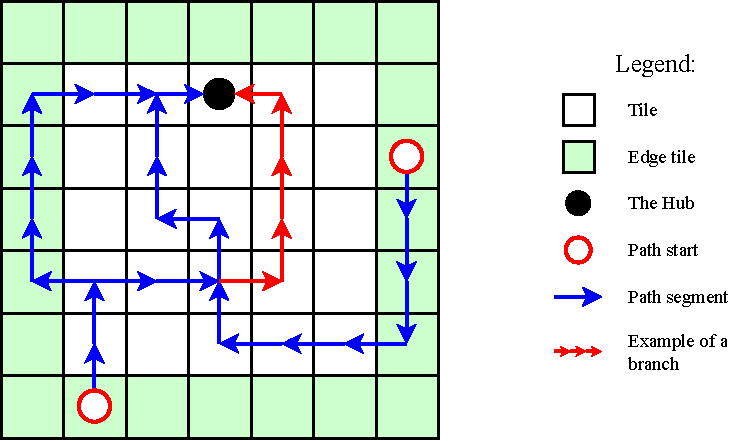
\includegraphics[width=0.7\textwidth]{img/Example path network.pdf}
    \caption{A path network in a $7\times7$ tile world.}
    \label{fig:path-network}
\end{center}

If tile $u$ can be reached from tile $t$ by going along $d$ path segments, we say the \textbf{path distance} from $t$ to $u$ is $d$.
Two tiles can have multiple different paths between them, however by requirement RP~\ref{RP:equal-distance}, all of these paths must have the same distance.
When $u$ is not reachable from $t$, they do not have a path distance.
The \textbf{path length} of a start dictates its path distance to the Hub.
For example, the path start on the bottom left of figure~\ref{fig:path-network} has path length 9.

\subsection{Hub Position and Path Starts} \label{sec:analysis-path-starts}

In the first stage of path generation, we need to select the tile the Hub will be on, and all the path starts.
This will be informed by the number of path starts we have to generate and their path lengths.

\head{Hub Position}{hub-pos}
First, we will select the Hub tile.
According to requirement RP\ref{RP:hub-pos}, it \enquote{should not be near the edge of the world, and it should be close to the center in levels with multiple paths}.
There aren't any more requirements, so we will simply select a random tile from tiles that are at most some distance from the center using the euclidean metric.
This distance will be the greatest for levels with one path start and decrease with each additional path start.

\head{Path Start Requirements}{path-start-req}
Now we select the path starts.
According to requirement RP\ref{RP:start-outside}, \enquote{paths start on tiles just outside the playable world, and the first path segment goes from the path start to the nearest tile in the playable world.}
However, other path segments are confined to the actual tiles of the world.
For simplicity, and to avoid edge cases when generating paths, we will pretend, that the paths start at an edge tile of the world, where the first path segment will end.

We will add this segment going over the edge only after the paths are generated.
This segment is uniquely determined anyway, except in the corners of the world, where we'll always select the one that makes the path go straight, as shown in figure~\ref{fig:real-path-starts}.
On the right are the pats as we think of them when generating, and on the left are the actual final paths.
The red circles represent the path starts, and the arrows represent the first segment of each path that only gets added at the end.

\begin{center}
    \captionsetup{type=figure}
    \begin{minipage}{.5\textwidth}
        \centering
        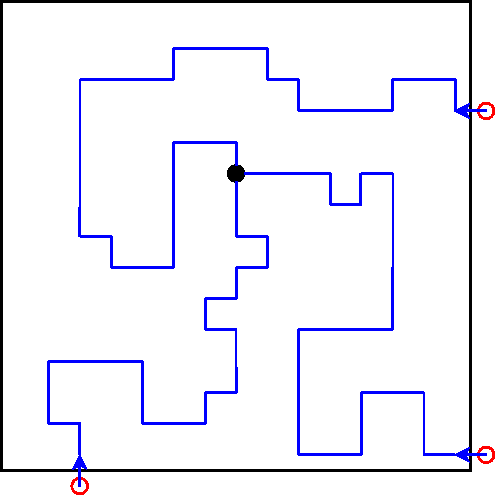
\includegraphics[width=0.95\textwidth]{img/path starts real.pdf}
    \end{minipage}%
    \begin{minipage}{.5\textwidth}
        \centering
        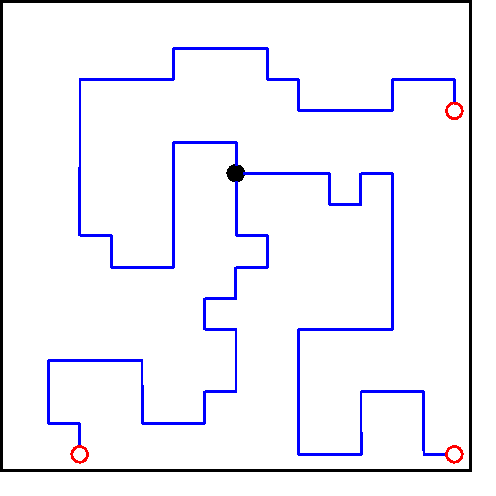
\includegraphics[width=0.95\textwidth]{img/path starts theory.pdf}
    \end{minipage}
    \caption{Real path starts compared to the ones we work with.}
    \label{fig:real-path-starts}
\end{center}

What tiles are valid for a path start with a given path length?
Each start must be at an edge tile, such that a path of the given length can go from it to the Hub.
It is easy to see that the minimum path distance between two tiles is their Manhattan distance.
So, we know that each start cannot be further from the Hub in Manhattan distance that its path length.

We can imagine creating a path backwards from the Hub by appending a segment at every step.
After the first step, the path starts on the neighboring tile of the Hub tile.
Both Manhattan distance and path distance from the tile to the Hub are 1.
After every step, the path distance increases by 1, changing its parity from odd to even or vice versa.
The Manhattan distance to the Hub either increases or decreases by 1, also changing its parity.
Thus, the parity of the path distance and Manhattan distance always match.
This means a path start with an even path length must be a tile with an even Manhattan distance to the Hub, and analogously for odd lengths.

In levels with more paths, we want the path starts to be spread out from each other, in order to cover the world with paths more evenly.
We can choose a minimum distance between the paths starts.
For levels with just one long path, we can also set a minimum distance from the Hub, so it starts further away from it and has more space to zigzag through the world.

\head{Selecting Path Starts}{select-path-starts}
To actually select the starts, we find all edge tiles, and separate them into two sets~--- each for one parity.
Then to select each start, we can use rejection sampling.
This means we take random tiles from the set of with the correct parity until we find one that satisfies all the conditions.
As long as the minimum distances between path starts and from the Hub are small enough, this approach always yields a valid list of path starts.
However, with stricter parameters it is possible that the first few starts invalidate all other start positions.
In that case we can use rejection sampling again~--- trying to randomly select lists of starts, until we get one that's valid.
If the failure rate was great enough, it would be wise to select a different algorithm, but our requirements are not very strict, so rejection sampling works fine.

\subsection{Generating the Main Paths}\label{sec:analysis-main-paths}

From the previous step, we have the Hub position and all the path starts.
Now we want to generate the main paths, which will serve as a template for the next steps.
These paths have to have the correct lengths and follow the requirements, which we set in section~\ref{sec:design-paths}.

We couldn't find many resources on procedurally generated paths.
There is a lot of research on generating road networks, mazes or dungeons.
Theoretically, we could use one of the many algorithms for generating mazes~\cite{MazeWiki}, and modify it to suit our needs.
However, it would be difficult to achieve what we need using an approach that was designed for something else.

We found one algorithm specifically designed for procedurally generating paths, called \emph{path chiseling} by Boris the Brave on his blog~\cite{PathChiseling1,PathChiseling2}.
This algorithm creates random paths on a tile grid by randomly blocking off individual tiles until only one path remains.
This is more promising, however we were unable to find a good way to modify it to generate paths of specific lengths with the properties we want.

Since many of our requirements are more like suggestions, we always want to fulfill them almost the best we can.
This means we can look at the task as an optimization problem: create the \emph{best looking} paths, given the requirements like length, no crossing etc.
Since we want the paths to be randomized, we don't need to find the optimum, we only need a random solution that is good enough.
Given this, we decided to generate the paths using an optimization technique called \emph{simulated annealing}.

\subsection{Simulated Annealing}\label{sec:analysis-simulated-annealing}

Simulated annealing can be used to find an approximation of the global optimum of an optimization problem, much faster than it would take to find the exact global optimum.
A great analysis of this technique can be found in the article \citetitle{SimulatedAnnealing}~\cite{SimulatedAnnealing}.
In this section, we will describe the technique, and in the next section~(\ref{sec:analysis-our-simulated-annealing}), we will use it to generate the paths we want.

The problems simulated annealing can be used for have to be formulated as follows:
\begin{quotation}
    From the set of all states $S$, find a state $s^*$ that minimizes the cost function $f \colon S \to \R$, given a neighbor function $n \colon S \to \mathcal{P}(S)$ which gives the \emph{neighbor states} of each state.
\end{quotation}
For example, to use simulated annealing to solve the \emph{travelling salesman problem}, each state is usually defined as a permutation of the cities to be visited.
The cost function then gives the length of the salesman's path, and the neighbor function gives all the states that can be acquired by swapping two cities in the original state.

The process of simulated annealing is described in pseudocode as algorithm~\ref{alg:simulated-annealing}.
It starts in an initial state $s_0$ and runs for $max\_steps$ steps.
For each step, a temperature $t$ is computed, slowly decreasing from $t_{initial}$ in the first step, to $t_{final}$ at the final step.
In each step, a random neighbor $s'$ of the current state $s$ is selected, and an acceptance probability $p$ is computed, based on the values of $f(s)$, $f(s')$ and the current temperature $t$.
The new state $s'$ is then set as the current state with probability $p$.

This acceptance probability function can be implemented however we see fit, however it should follow these rules:
It always accepts a better new state ($s'$ such that $f(s') < f(s)$), but it can also give a non-zero probability when the new state is worse that the current state ($f(s') > f(s)$).
The probability to accept a worse new state decreases with decreasing temperature.
The acceptance probability of state $t$ cannot be greater than the probability of $u$ when $t$ is worse than $u$ ($f(t) > f(u)$).

\begin{algorithm}[H]
    \caption{Simulated annealing}
    \label{alg:simulated-annealing}
    \begin{algorithmic}[1]
        \State $s \gets s_0$
        \For{$k$ from $0$ to $max\_steps-1$}
        \State $t \gets$ \Call{Lerp}{$t_{initial}$, $t_{final}$, $k/(max\_steps-1)$}
        \State $s' \gets$ random neighbor from $n(s)$
        \State $p \gets$ \Call{AcceptanceProbability}{$f(s)$, $f(s')$, $t$}
        \State with probability $p$: $s \gets s'$
        \EndFor\\
        \Return $s$
        \Statex
    \end{algorithmic}
\end{algorithm}

It is easy to see that if the algorithm never accepted states which are worse than the current state, it would gradually reach a local optimum.
Since it also accepts worse states, it can move away from the local optimum and hopefully end up in a better one.
The probability to accept a worse state gradually decreases with the decreasing temperature.
So at the start, when the temperature is high, the algorithm explores the search space a lot, but as the temperature decreases, it is less and less likely to escape from the local optimum it finds.
Since the exploration prioritizes better states, it is more likely to lead the algorithm to a better optimum than a worse one.

\subsection{Generating Paths using Simulated Annealing}\label{sec:analysis-our-simulated-annealing}

To use simulated annealing to optimize paths, we need to formulate our task as an optimization problem that simulated annealing can solve.
We need to define what is a state, a cost function and a neighbor function.

\head{States}{sa-states}
Each state is a path network composed of one path for each path start.
We will represent each path by a sequence of tiles the path goes through.
Two consecutive tiles in the sequence must be neighbors.
Additionally, each path starts at the given path start, has the correct length, and ends at the Hub tile.
We chose this representation to make it easy to generate neighbor states.
Notice, that we don't check for any intersections and a path can visit one tile multiple times.
This is because the state is going to change only by a small amount at every step.
If we banned intersections, we would lose too much freedom during the simulated annealing, and the final state would always end up close to the initial state.

\head{Neighbor States}{sa-neighbors}
We decided that two states are neighbors when they differ only by one tile.
To generate the set of all neighbors, we have to find all the ways to change one tile in the state to a different tile, such that the result is still a valid state.

For a state to be valid, we require that each path starts with the path start and ends with the Hub tile.
This means that the first and last tile of every path can never change.
For each other tile, there aren't many options on how to change it.
All these options, up to symmetry, are illustrated in figure~\ref{fig:path-tile-swaps}.
The tiles in the sequence are drawn as circles connected by arrows that show their order in the sequence.
The tile we plan to change is drawn as a red circle.
Additionally, we draw the tiles which go before and after it in the sequence.
These are the only tiles that determine the possible changes.

When the tiles form a straight line, no change is possible.
When they form a right angle, one change is possible.
And when the same tile comes before and after, 3 changes are possible.

\begin{center}
    \captionsetup{type=figure}
    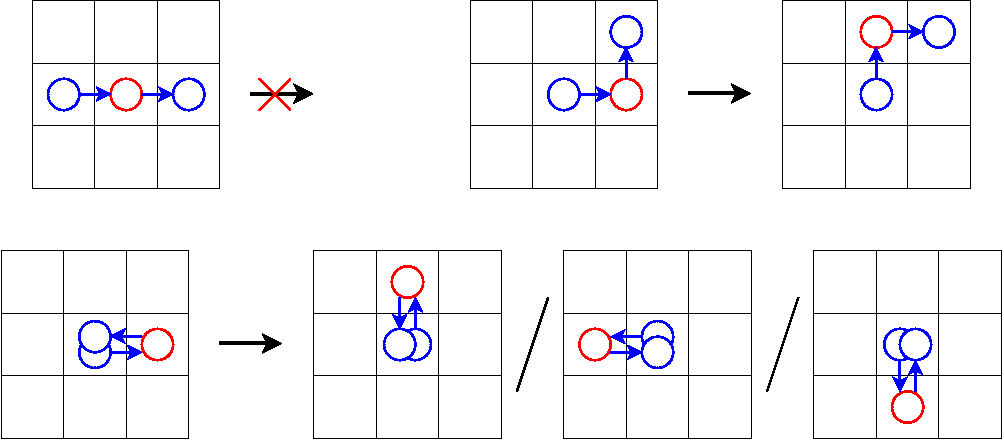
\includegraphics[width=0.7\textwidth]{img/SA tile swaps.pdf}
    \caption{All the possible tile changes.}
    \label{fig:path-tile-swaps}
\end{center}

\head{Cost function}{sa-cost-function}
Now we select a cost function that gives a better score to paths that are more desirable.
Since we want the paths to spread out, we can calculate for each tile of the world what we call a \emph{crowding penalty}.
Each time a tile appears in the state, it's crowding penalty increments by 1, and all other tiles get a lower penalty decreasing with euclidean distance.
This way, the tiles that get visited the most times get the highest crowding penalty.
A tile can be substantially crowded even when no path goes through it just because there is a lot of paths around it.

We will denote the crowding penalty that tile $t$ gets from tile $u$ as $c(t,u)$.
The total crowding penalty from tiles in state $s$ for a given tile $t$ is then $c_t(t,s) = \sum_{u \in s} c(t,u)$.

We also add a big crowding penalty to the tiles along the edge of the world, which gradually decreases as we go away from the edge.
This is to push the paths away from the edges, as that is undesirable by requirement RP\ref{RP:undesirable}.
We will denote the crowding penalty that tile $t$ gets from its closeness to the edge as $c_e(t)$.

We define the cost function of a state $s$ as the sum of the crowding penalties of each tile in the state:
\begin{equation*}
    f(s) = \sum_{t \in s} \left(c_e(t) + c_t(t)\right) = \sum_{t \in s} \left(c_e(t) + \sum_{u \in s} c(t,u) \right)
\end{equation*}
This is an obvious choice, because we want each tile to be crowded as little as possible.
So, a state with less crowded tiles has a lower cost, and a state with more crowded tiles has a higher cost.

However, we can just calculate the relative improvement $r_i = f(s) - f(s')$ between the current state $s$ and the new state $s'$ to save on computation.
The relative improvement still gives us enough information to create a good acceptance probability function, but it is simple to compute, because $s$ and $s'$ share most of their tiles.

For $s'$ obtained by changing tile $v$ in $s$ to $w$, we can calculate $r_i$ as:
\begin{equation*}
    r_i = c_e(v) - c_e(w)  + 2 c_t(v,s) - 2 c_t(w,s) + 2c(w,v) - 2
\end{equation*}
We prove this in section~\ref{sec:analysis-proof-improvement}.
This can be computed in $O(1)$ time if we keep the $c_t(t,s)$ of every tile $t$ in the world.
We have to keep all $c_t$ updated when we change the current state to the new state.
This update is simple for each tile $t$:
\begin{equation*}
    c_t(t,s') = c_t(t,s) - c(t,v) + c(t,w)
\end{equation*}

\head{Initial State}{sa-initial-state}
Now, with the problem formulated, we still need to fill in a few details to be able to solve it.
First, we need to produce an initial state.
This is not trivial, because of our constraints on what's considered a valid state.
Namely, every path has to be the correct length.
However, we can easily produce a valid initial state using a random walk from each path start.

The algorithm starts on the path start tile, and adds it to the state as the first path tile of this path.
Then it moves to a random neighbor and appends it to the sequence.
This is repeated until it creates a path of the correct length.
However, we need to ensure that the path ends at the Hub.
To achieve this, we just make the algorithm never select a tile that is further away from the Hub in Manhattan distance than the remaining length of the path.

\head{Acceptance Probability Function}{sa-acceptance-probability-function}
Next, we need to select an acceptance probability function that works well for this problem.
We don't compute the cost of the current state $f(s)$ and the cost of the new state $f(s')$ separately, instead we compute only the relative improvement $r_i = f(s) - f(s')$.
This means that the function will decide on the probability only based on the relative improvement and the temperature.
The function needs to fulfill the requirements outlined in the previous section~\ref{sec:analysis-simulated-annealing}.
The most straight-forward function is simply $r_i - t$.
This function can return values greater than 1 and less than 0, this does not matter, because when testing the probability, these values get treated as 1, respectively 0.

Is this the best function for this problem?
We don't know, but it performed well in our testing, so we kept it.

\head{Intersection Untwisting}{sa-intersections}
However, when we use simulated annealing with these parameters, it still sometimes produces paths that intersect.
This is because it is difficult for the algorithm to fix a loop in the path, as shown on the left in figure~\ref{fig:untwisting-paths}.
It would first have to bring many path tiles closer together, in order to let them cross over each other.
This is the sort of problem simulated annealing is supposed to be able to overcome.
However, we can help it by adding a step that just \emph{untwists} crossings by reversing the section of the path that forms a loop, as shown in the figure.
This still leaves two identical tiles, but now, simulated annealing can drive these apart without any issue.

\begin{center}
    \captionsetup{type=figure}
    \begin{tikzpicture}
        \draw[step=1.0,black,thin] (0,0) grid (4,4);
        \draw[step=1.0,black,thin] (6,0) grid (10,4);
        \begin{scope}[blue,very thick,decoration={
                        markings,
                        mark=between positions 0.25cm and -0.05cm step 0.5cm with {\arrow{>}};
                    }]
            \draw[postaction={decorate},shift={(0.5,0.5)}] (-1,1)--(3,1);
            \draw[white,line width=4pt,shift={(0.5,0.5)}] (1,0.6)--(1,1.4);
            \draw[postaction={decorate},shift={(0.5,0.5)}] (3,1)--(3,3)--(1,3)--(1,-1);
            \draw[postaction={decorate},shift={(0.5,0.5)}] (5,1)--(6.95,1.05);
            \draw[postaction={decorate},shift={(0.5,0.5)}] (6.95,1.05)--(7,3);
            \draw[postaction={decorate},shift={(0.5,0.5)}] (7,3)--(9,3)--(9,1);
            \draw[postaction={decorate},shift={(0.5,0.5)}] (9,1)--(7.05,0.95);
            \draw[postaction={decorate},shift={(0.5,0.5)}] (7.05,0.95)--(7,-1);
        \end{scope}
        \draw[->,very thick,shift={(0.5,0.5)}] (4,1.5) -- (5,1.5);
    \end{tikzpicture}
    \caption{Untwisting a self-intersecting path.}
    \label{fig:untwisting-paths}
\end{center}

This modification of the state is valid, because the length of the path doesn't change.
However, we cannot untwist crossings between two different paths, because that could change their lengths.
This means that we should take special care to not produce an initial state where two different paths cross.
We can achieve this by calculating crowding penalties while creating the initial state.
Then, when the random walk algorithm selects a random neighbor to move to, we make it prefer the neighbors with a lower crowding penalty.
Because we don't mind self-intersections, we don't add the crowding penalties from the nodes of the path the algorithm is currently creating.
We add them only when the path is complete.

Still, the algorithm sometimes fails in creating a valid path network.
In case no valid network is generated, we can restart the path generation algorithm, including picking new starting positions.

In figure~\ref{fig:simulated-annealing}, we can see how the paths evolve over time as the temperature decreases.
\begin{center}
    \captionsetup{type=figure}
    \begin{minipage}{.5\textwidth}
        \centering
        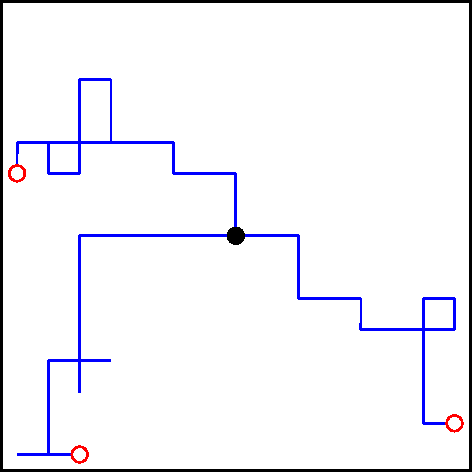
\includegraphics[width=0.95\linewidth]{img/SA initial state.pdf}
        \subcaption{Initial state ($t_{initial} = 2.5$)}
    \end{minipage}%
    \begin{minipage}{.5\textwidth}
        \centering
        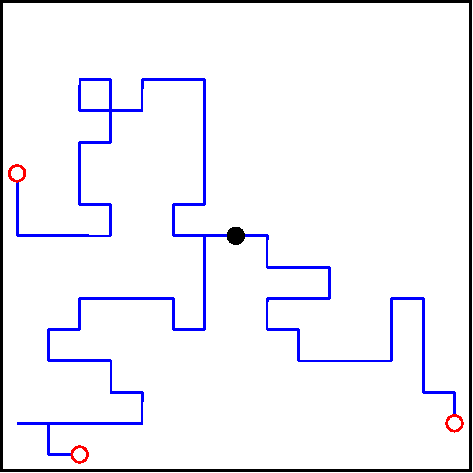
\includegraphics[width=0.95\linewidth]{img/SA temp 2.pdf}
        \subcaption{$t = 2$}
    \end{minipage}\\
    \begin{minipage}{.5\textwidth}
        \centering
        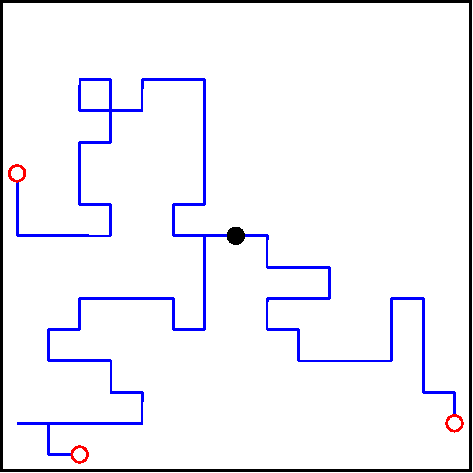
\includegraphics[width=0.95\linewidth]{img/SA temp 1.5.pdf}
        \subcaption{$t = 1.5$}
    \end{minipage}%
    \begin{minipage}{.5\textwidth}
        \centering
        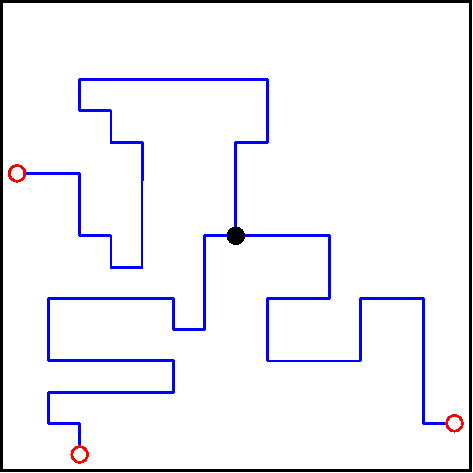
\includegraphics[width=0.95\linewidth]{img/SA final.pdf}
        \subcaption{Result ($t_{final} = 1$)}
    \end{minipage}
    \caption{Evolution of paths during simulated annealing.}
    \label{fig:simulated-annealing}
\end{center}

\subsection{Simplifying the Relative Improvement Calculation}\label{sec:analysis-proof-improvement}

In paragraph~\nameref{head:sa-cost-function} of the previous section, we defined the cost function we will use and its components:
The cost function for state $s$ is defined as follows:
\begin{equation*}
    f(s) = \sum_{t \in s} \left(c_e(t) + \sum_{u \in s} c(t,u) \right)
\end{equation*}
Where $c(t,u)$ is the crowding penalty that tile $t$ gets from its distance to tile $u$, and $c_e(t)$ is the crowding penalty tile $t$ gets from its distance to the edge of the world.
The total crowding penalty from tiles in state $s$ for a given tile $t$ is then $c_t(t,s) = \sum_{u \in s} c(t,u)$.
We also stated that we will only calculate the relative improvement $r_i = f(s) - f(s')$ between the current state $s$ and the new state $s'$.

In this section, we show that the relative improvement $r_i = f(s) - f(s')$ for $s'$ obtained by changing tile $v$ in $s$ to $w$ can be calculated as follows:
\begin{equation*}
    r_i = c_e(v) - c_e(w)  + 2 c_t(v,s) - 2 c_t(w,s) + 2c(w,v) - 2
\end{equation*}

We start by substituting the definition for the cost function $f$.
\begin{align*}
    r_i & = f(s) - f(s')                                                                                                                \\
        & = \sum_{t \in s} \left(c_e(t) + \sum_{u \in s} c(t,u) \right) - \sum_{t \in s'} \left(c_e(t) + \sum_{u \in s'} c(t,u) \right)
\end{align*}
Now we separate $v$ from $s$ and $w$ from $s'$.
\begin{align*}
     & = \sum_{t \in s} \left(c_e(t) + c(t,v) + \sum_{u \in s - v} c(t,u)\right) - \sum_{t \in s'} \left(c_e(t) + c(t,w) + \sum_{u \in s' - w} c(t,u) \right) \\
     & = \left(c_e(v) + c(v,v) + \sum_{u \in s - v} c(v,u)\right) + \sum_{t \in s - v} \left(c_e(t) + c(t,v) + \sum_{u \in s - v} c(t,u)\right)               \\
     & \ - \left(c_e(w) + c(w,w) + \sum_{u \in s' - w} c(w,u) + \sum_{t \in s' - w} \left(c_e(t) + c(t,w) + \sum_{u \in s' - w} c(t,u) \right) \right)        \\
    \intertext{We use that $s - v = s' - w$, and we name $q$ the set of tiles both states have in common.}
     & = c_e(v) + c(v,v) + \sum_{u \in q} c(v,u) + \sum_{t \in q} \left(c_e(t) + c(t,v) + \sum_{u \in q} c(t,u)\right)                                        \\
     & \ - \left(c_e(w) + c(w,w) + \sum_{u \in q} c(w,u) + \sum_{t \in q} \left(c_e(t) + c(t,w) + \sum_{u \in q} c(t,u) \right)\right)                        \\
     & = c_e(v) + c(v,v) + \sum_{u \in q} c(v,u) + \sum_{t \in q} c_e(t) + \sum_{t \in q} c(t,v) + \sum_{t \in q} \sum_{u \in q} c(t,u)                       \\
     & \ - \left(c_e(w) + c(w,w) + \sum_{u \in q} c(w,u) + \sum_{t \in q} c_e(t) + \sum_{t \in q} c(t,w) + \sum_{t \in q} \sum_{u \in q} c(t,u)\right)        \\
     & = c_e(v) + c(v,v) + \sum_{u \in q} c(v,u) +  \sum_{t \in q} c(t,v)                                                                                     \\
     & \ - \left(c_e(w) + c(w,w) + \sum_{u \in q} c(w,u) + \sum_{t \in q} c(t,w) \right)                                                                      \\
    \intertext{The function $c$ is symmetric, because it depends only on the distance between the tiles, which is symmetric, so we get:}
     & = c_e(v) + c(v,v) + 2 \sum_{t \in q} c(v,t) - \left(c_e(w) + c(w,w) + 2 \sum_{t \in q} c(w,t) \right)                                                  \\
    \intertext{The crowding a tile inflicts to itself is 1, so $c(v,v) = c(w,w)$.}
     & = c_e(v) - c_e(w)  + 2 \sum_{t \in q} c(v,t) - 2 \sum_{t \in q} c(w,t)                                                                                 \\
    \intertext{We can add the terms $2c(v,v) - 2c(v,v) + 2c(w,v) - 2c(w,v)$ because they sum to zero:}
     & = c_e(v) - c_e(w)  + 2 \sum_{t \in q} c(v,t) - 2 \sum_{t \in q} c(w,t)                                                                                 \\
     & \ + 2c(v,v) - 2c(v,v) + 2c(w,v) - 2c(w,v)                                                                                                              \\
    \intertext{And we collect the sums to sum over the elements of $s$.}
     & = c_e(v) - c_e(w)  + 2 \sum_{t \in s} c(v,t) - 2 \sum_{t \in s} c(w,t) - 2c(v,v) + 2c(w,v)                                                             \\
     & = c_e(v) - c_e(w)  + 2 c_t(v,s) - 2 c_t(w,s) - 2c(v,v) + 2c(w,v)                                                                                       \\
     & = c_e(v) - c_e(w)  + 2 c_t(v,s) - 2 c_t(w,s) + 2c(w,v) - 2
\end{align*}
$\hfill\square$

So we see that the equality holds, letting us compute the relative improvement more efficiently.

\subsection{Final Paths}\label{sec:analysis-final-paths}

Now that we have generated the main paths, we just have to generate the side branches.
The world generation steps that come after have to make sure to not block the paths we have generated.
However, we don't want to constrain them with the whole path network.
Since we don't have requirements on the minimum side branch count or their lengths, it is enough to ensure the paths we generated in the previous step get preserved.
We can generate the rest of the world first, and only then make extra paths where they fit.
We don't want the branching to feel the same in every level.
This lets us use the randomness of the world generation instead of needing to introduce more in this stage.

Due to this decision, this step will start with an already generated terrain and obstacles, as described in sections~\ref{sec:analysis-terrain-generation} and~\ref{sec:analysis-obstacles}.
These steps respect the original paths, but they will cause other tiles or edges between them to be blocked, as shown in figure~\ref{fig:paths-world}.
Here, we can see the original paths on the left.
On the right, we can see tiles blocked by obstacles as gray squares with black edges.
Additionally, some edges between tiles are also blocked, usually because the two tiles are at different height levels, separated by a cliff.
These are the remaining black lines.

\begin{center}
    \captionsetup{type=figure}
    \begin{minipage}{.5\textwidth}
        \centering
        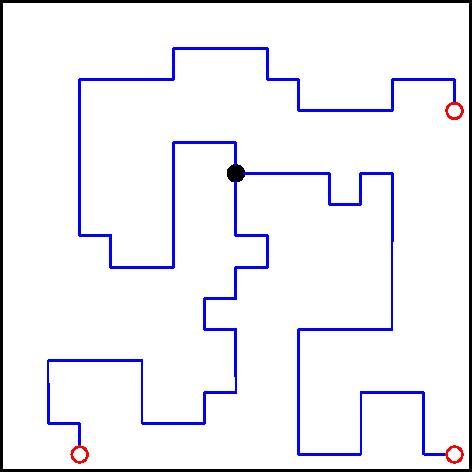
\includegraphics[width=0.95\textwidth]{img/Generated Paths.pdf}
    \end{minipage}%
    \begin{minipage}{.5\textwidth}
        \centering
        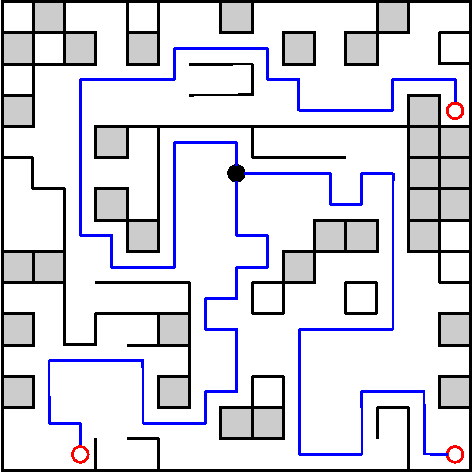
\includegraphics[width=0.95\textwidth]{img/Paths and world.pdf}
    \end{minipage}
    \caption{Blocked edges and tiles after generating the terrain and obstacles.}
    \label{fig:paths-world}
\end{center}

Now, how do we actually generate the path network?
There are so many blocked edges that we want to add all the valid branches we find, up to the maximum number of branches decided by the map generator (see section~\ref{sec:analysis-procedural-generation}).
To do this, we will use depth first search, but we will add a few heuristics to produce better paths.
To decide on these heuristics, we will set a few more requirements:
We still want the paths to be spread out, but we would prefer the paths to go straight if possible.

However, we would also like to somehow capture the shape of the paths that were optimized during the previous stage.
We could simply make the first path from each start be identical to the original path.
We would like multiple paths to sometimes join together, which we cannot do without changing them.
To achieve this, we add a rule for every tile with a path: if an original path also went through it, its path distance must be the same as the original path distance.
This way, the path segments of any new path will be distributed similarly to the original path, since they have to cross at every choke point.
This is illustrated in figure~\ref{fig:respect-originals}.
On the left are the original paths, and on the right are randomly generated paths which respect the rule.
The tiles where the random paths would intersect the original paths are marked with a blue circle.

\begin{center}
    \captionsetup{type=figure}
    \begin{minipage}{.5\textwidth}
        \centering
        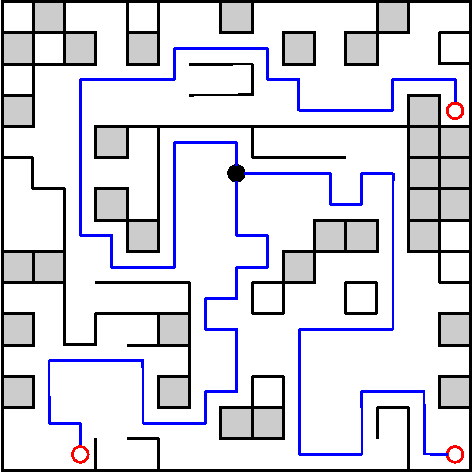
\includegraphics[width=0.95\textwidth]{img/Paths and world.pdf}
    \end{minipage}%
    \begin{minipage}{.5\textwidth}
        \centering
        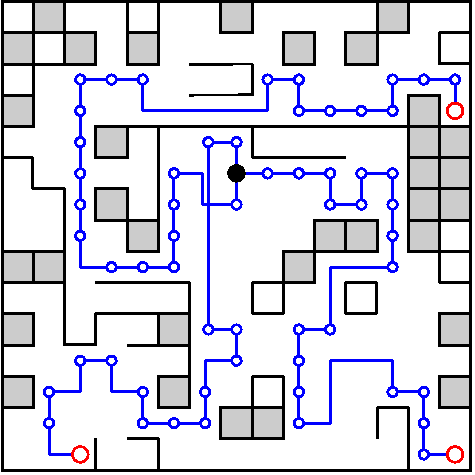
\includegraphics[width=0.95\textwidth]{img/Rnadom but respecting the originals.pdf}
    \end{minipage}
    \caption{Randomly generated paths which respect the original path distances.}
    \label{fig:respect-originals}
\end{center}

We need to make sure the paths we produce are the correct length and respect the required original path distances.
We can save a lot of time by precomputing the minimum distance each tile can have.
This way the algorithm can avoid tiles from which it's impossible to finish a path of the correct length.
For this, we can do a breadth first search from the Hub tile, and we restrict the original path tiles to only \enquote{be found} at the right time and not sooner.
The result can be seen in figure~\ref{fig:path-distances}.
We will call these distances the \emph{minimum distances}.

\begin{center}
    \captionsetup{type=figure}
    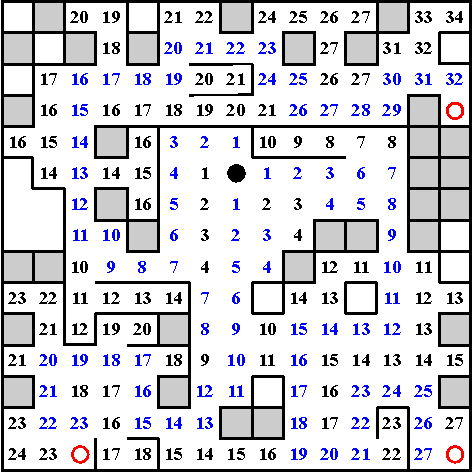
\includegraphics[width=0.5\textwidth]{img/Path Distances.pdf}
    \caption{Calculated minimum distances.}
    \label{fig:path-distances}
\end{center}

Now we finally run the depth first search, one path by one.
The algorithm keeps a stack of \emph{path prototypes}.
These are paths, which start at the start tile, but have not reached the Hub yet.
At the start, the stack contains only the path prototype with only the start position as its only element.
At every step, the algorithm pops the last prototype from the stack, finds all valid one-step continuations of the current paths, and adds those to the stack.

Valid continuations are the neighbors of the last tile of the current path prototype that aren't blocked.
Additionally, they have to have a minimum distance that is less than or equal to the remaining length of this path prototype.
The valid continuations are ordered such that the best option will be put onto the stack last, so it gets popped in the next step.
The best option is always the one that goes straight, and the rest is ordered by the same crowding penalty as in paragraph~\nameref{head:sa-cost-function} of section~\ref{sec:analysis-our-simulated-annealing}.

Once the algorithm reaches the Hub or an already existing path, it checks whether it is valid to finish the current path.
First, it must have the correct remaining length to produce a valid path.
When it connects to the Hub, the remaining length must be 0, and for connecting to an existing path, the remaining length must match the path distance of that tile.
Additionally, as per requirement RP\ref{RP:branch}: \enquote{every branch must go through at least one tile that is not adjacent to any already existing path}.

If this check fails, the algorithm does not mark this branch, it pops the last item from the stack and continues from there.
If the check succeeds, it marks the new path section and updates the crowding penalties to take the new path section into account.
Then it continues by making another branch.

However, the last path prototype on the stack will share most of its tiles with the branch we just found.
We want the branches be separated from each other as much as possible.
To minimize the shared section, we take the path prototype from the opposite end of the stack.
So, in reality, we won't use a stack, but a double ended queue.
The entire search is described in pseudocode as algorithm~\ref{alg:path-finalizing}.

\begin{algorithm}[H]
    \caption{Finalizing paths}
    \label{alg:path-finalizing}
    \begin{algorithmic}[1]
        \ForEach{path start $start$}
        \State $stack$.\Call{PushLast}{path prototype containing only $start$}
        \State $success \gets$ \mono{false}
        \Statex
        \While{$stack$ is not empty}
        \If{$success$}
        \State $p \gets stack$.\Call{PopFirst}{}
        \Else
        \State $p \gets stack$.\Call{PopLast}{}
        \EndIf
        \Statex
        \If{last tile in $p$ contains a path or the Hub}
        \State $success \gets$ \Call{TryFinishPath}{$p$}
        \Else
        \State $success \gets$ \mono{false}
        \ForEach{tile $c$ from \Call{GetValidContinuations}{$p$}}
        \State $stack$.\Call{PushLast}{$p$ extended by $c$}
        \EndFor
        \EndIf
        \EndWhile
        \EndFor
        \Statex
    \end{algorithmic}
\end{algorithm}

With this ordering of valid continuations, the algorithm usually reaches the Hub too soon, and then it has to backtrack many times before producing a path that is the right length.
To fix this, we prioritize above all the tiles with minimum distance exactly equal to the remaining length.
The results of the algorithm are displayed on the right in figure~\ref{fig:final-paths}, compared to the initially generated paths on the left.
Segments that have changed are highlighted in red.

\begin{center}
    \captionsetup{type=figure}
    \begin{minipage}{.5\textwidth}
        \centering
        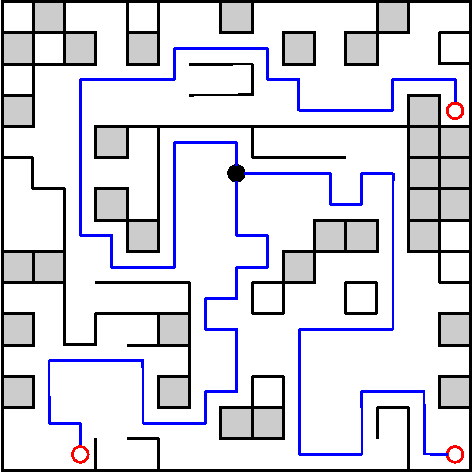
\includegraphics[width=0.95\textwidth]{img/Paths and world.pdf}
    \end{minipage}%
    \begin{minipage}{.5\textwidth}
        \centering
        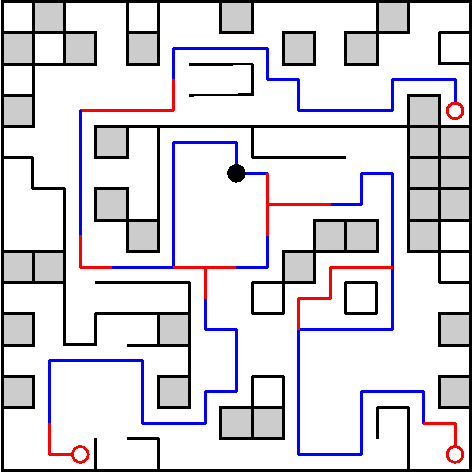
\includegraphics[width=0.95\textwidth]{img/Final Paths.pdf}
    \end{minipage}
    \caption{Final paths compared to the originally generated paths.}
    \label{fig:final-paths}
\end{center}

\section{Terrain Generation}\label{sec:analysis-terrain-generation}

There are many techniques we could use for generating the terrain.
However, we have pretty strict requirements for the terrain generation.
We need to make sure the paths we have generated in the previous step are not blocked by terrain features like cliffs.
We also want the algorithm to be able to generate different-looking terrain types.

This led us to a variant of a procedural generation algorithm called \emph{model synthesis}, originally developed by \Citeauthor{ModelSynthesis}~\cite{ModelSynthesis}.
The discrete version of this algorithm is better known by the name \emph{wave function collapse} (or~WFC in short), popularized by \Citeauthor{WFC} on GitHub~\cite{WFC}.
Model synthesis is more general and focuses more on 3D models, whereas WFC applies the same concepts to generating 2D pixel art and tile maps.
Since the name \enquote{wave function collapse} is more popular, we will use it in the rest of this thesis, even though it's not the name of the algorithm that came first.

We chose WFC, because it can generate randomized terrain, whilst fully respecting the initial constraints we give it.
To see how this works, we will explain the algorithm first.

\subsection{Wave Function Collapse}

The original intent behind the algorithm is to replicate the structure of an example on a larger scale, making sure that the output is locally similar to the input, as shown in figure~\ref{fig:wfc-example}.
We will limit our examples to 2-dimensional grids of tiles, however this algorithm works in more dimensions.

\begin{center}
    \captionsetup{type=figure}
    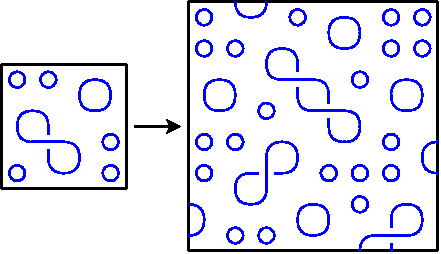
\includegraphics[width=0.5\textwidth]{img/WFC Example.pdf}
    \caption{Example input and output of the wave function collapse algorithm.}
    \label{fig:wfc-example}
\end{center}

The first step of the algorithm is to extract from the input which features can appear next to each other.
The algorithm creates a set of \emph{modules}\footnote{This is a naming convention used in an article by \Citeauthor{WFCMarian}~\cite{WFCMarian}.}, which are the building blocks the output will be built from.
Each module comes with a set of constraints on its neighbors.
The main portion of the algorithm then builds the output from these modules, such that all the constraints are satisfied, and each module appears in the output with a similar frequency to the input.
However, we will create the modules for our generator by hand, including their constraints, in order to have greater control over the generated result.
In figure~\ref{fig:wfc-modules}, we can see a set of 7 modules and the resulting output, given only the constraint that the edges of directly adjacent modules must match.

\begin{center}
    \captionsetup{type=figure}
    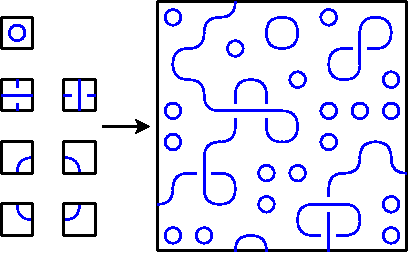
\includegraphics[width=0.5\textwidth]{img/WFC modules.pdf}
    \caption{Example output of WFC, using the modules on the left and only the constraint that their edges must match.}
    \label{fig:wfc-modules}
\end{center}

We call each spot in the output where a module is supposed to be a \emph{slot}.
Each slot keeps track of all the modules that can be placed in it.
At the start of the main part of the algorithm, all slots are initialized with all the modules.
Figure~\ref{fig:wfc-initial} shows a visualization of this state.
Then the algorithm repeats two actions: collapse a slot, propagate constraints.
To collapse a slot, the algorithm removes all possible modules from the slot except for one, chosen at random.

Then it has to propagate constraints, which means that it removes from each slot all the modules which can no longer be placed there.
For example, in figure~\ref{fig:wfc-step-1} we see that a slot has collapsed to a module which has a line on each edge.
Thus, the algorithm removes from the neighboring slots (marked in red) all modules which don't have a line at the corresponding edge.
After propagating constraints, the algorithm collapses another slot and so on.

\begin{center}
    \captionsetup{type=figure}
    \begin{minipage}{.31\textwidth}
        \centering
        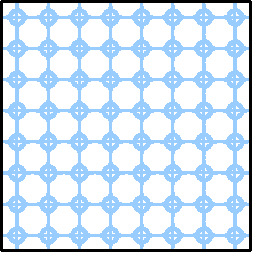
\includegraphics[width=0.95\linewidth]{img/WFC initial state.pdf}
        \subcaption{Initial state} \label{fig:wfc-initial}
    \end{minipage}%
    \begin{minipage}{.31\textwidth}
        \centering
        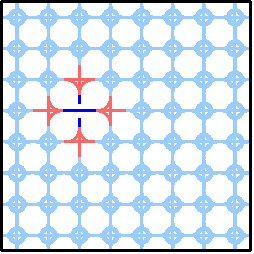
\includegraphics[width=0.95\linewidth]{img/WFC step 1.pdf}
        \subcaption{First step} \label{fig:wfc-step-1}
    \end{minipage}%
    \begin{minipage}{.31\textwidth}
        \centering
        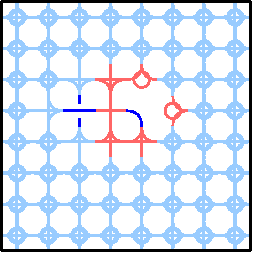
\includegraphics[width=0.95\linewidth]{img/WFC step 2.pdf}
        \subcaption{Second step} \label{fig:wfc-step-2}
    \end{minipage}
    \caption{Two steps of wave function collapse.}
    \label{fig:wfc-steps}
\end{center}

In figure~\ref{fig:wfc-step-2}, we can see an interesting situation after collapsing a second slot.
The slot between the collapsed slots can still contain two possible modules, however both of them have a line at the top and bottom edges.
This means that the algorithm also has to propagate to the neighbors of this tile that they have to have lines at the corresponding edges.
A change in one slot can affect slots even very far away from it.

This process repeats until all slots are collapsed, at which point we have successfully generated the output.
This process is summarized as algorithm~\ref{alg:wfc}.
We left out one detail: which element does \textsc{Pop} select?
This does not matter for the overall function of the algorithm, and it will be further discussed in section~\ref{sec:analysis-our-wfc}.
We will call this algorithm WFC, even though it differs from both WFC by Gumin and Merrell's model synthesis.
The only notable difference is that we skip the feature extraction step, and the algorithm takes as input the modules directly.

\begin{algorithm}[H]
    \caption{A na\"{i}ve version of wave function collapse}
    \label{alg:wfc}
    \begin{algorithmic}[1]
        \ForEach{slot $s$ in output} \Comment{Initialize all slots.}
        \State $s.modules \gets all\_modules$
        \EndFor
        \Statex
        \State $uncollapsed \gets$ all slots
        \While{$uncollapsed$ is not empty}
        \State $s \gets uncollapsed$.\Call{Pop}{} \Comment{Collapse a slot.}
        \State $s.modules \gets \{$random module from $s.modules\}$
        \Statex
        \State $to\_update \gets$ neighbors of $s$ \Comment{Propagate constraints.}
        \While{$to\_update$ is not empty}
        \State $u \gets to\_update$.\Call{Pop}{}
        \Statex
        \State $changed \gets$ \mono{false}
        \ForEach{module $m$ in $u.modules$} \Comment{Remove invalid modules.}
        \If{not \Call{IsValid}{$m$}}
        \State $u.modules \gets u.modules - m$
        \State $changed \gets$ \mono{true}
        \EndIf
        \EndFor
        \Statex
        \If{$changed$} \Comment{If $u$ changed, enqueue its neighbors.}
        \State $to\_update \gets to\_update\,\cup$ neighbors of $u$
        \EndIf
        \Statex
        \EndWhile
        \EndWhile
        \Statex
    \end{algorithmic}
\end{algorithm}

However, it is possible for the algorithm to create a slot with no valid module.
In that case, it is no longer possible to create a valid output.
We call this situation a \emph{conflict}.
An example can be seen in figure~\ref{fig:wfc-backtracking}.
If we look at WFC as a \emph{constraint satisfaction problem} solver, we can see that the constraint propagation only ensures \emph{arc-consistency}, which is not enough to rule out conflicts.
This is concisely explained in the Wikipedia article on local consistency~\cite{LocalConsistencyWiki}.

We called algorithm~\ref{alg:wfc} na\"{i}ve, because it is unable to deal with any conflicts.
What can we do to always produce a result, even when a conflict happens?
One option is to simply restart the algorithm.
For sufficiently small outputs, conflicts should be rare enough, only needing a few restarts.

Another option is to use backtracking.
Whenever the algorithm runs into a contradiction after collapsing a slot, it returns to the state before collapsing.
Additionally, it removes the module the slot collapsed to from its valid options, because it now knows it causes to a conflict.
The state after backtracking is illustrated in fig~\ref{fig:wfc-after-backtracking}.
This way, the algorithm can continue generating without getting rid of all its progress.

\begin{center}
    \captionsetup{type=figure}
    \begin{minipage}{.31\textwidth}
        \centering
        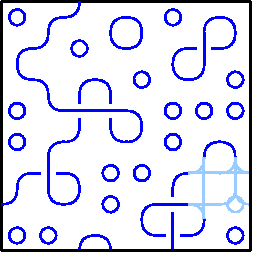
\includegraphics[width=0.95\linewidth]{img/WFC backtracking before.pdf}
        \subcaption{Before collapsing} \label{fig:wfc-before-backtracking}
    \end{minipage}%
    \begin{minipage}{.31\textwidth}
        \centering
        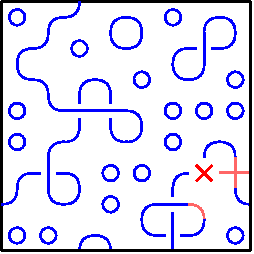
\includegraphics[width=0.95\linewidth]{img/WFC backtracking dead end.pdf}
        \subcaption{After collapsing} \label{fig:wfc-dead-end}
    \end{minipage}%
    \begin{minipage}{.31\textwidth}
        \centering
        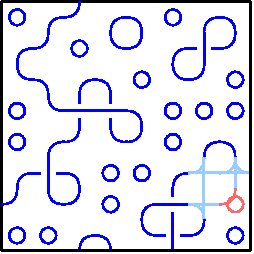
\includegraphics[width=0.95\linewidth]{img/WFC backtracking after.pdf}
        \subcaption{After backtracking} \label{fig:wfc-after-backtracking}
    \end{minipage}
    \caption{Conflicts and backtracking in WFC. The red cross marks a slot with no valid modules.}
    \label{fig:wfc-backtracking}
\end{center}

\subsection{Advantages and Disadvantages of WFC}

The main advantage of WFC is that it offers a lot of control over the generated world.
That's ultimately why we chose to use it.
We always know what features can appear in the world, because we explicitly select them as building blocks of the terrain.
We can also freely constrain the world that we are generating.
For example, we can force the generator to not block the paths we've generated in the previous stage, and we can force the tile with the Hub to be flat.
We also force a random tile to be at the lowest height level and another to be at the highest.

However, WFC has some disadvantages when used as a terrain generator.
First, it is very slow.
Even the na\"{i}ve implementation has to do a lot of work for each slot in the world.
However, the real problem are the conflicts.
Merrell shows in section 3.3.5 of their thesis that deciding whether an incomplete output is consistent, i.e., it can be completed without running into contradictions, is an NP-complete problem.
This necessarily means that WFC cannot run in polynomial time for all inputs, assuming P~$\neq$~NP.

The real problem is that the algorithm usually does run into contradictions, and the larger the generation task, the more likely it is to run into a contradiction.
This is especially bad for online generation of infinite worlds, because we can't simply restart and generate a new world after the player has already seen a part of it.
Backtracking also doesn't solve this issue, because the algorithm can collapse a slot in a way that is guaranteed to cause a contradiction, and then do arbitrarily many more steps before finally running into it.
Of course, there are ways to circumvent this issue, namely by making the individual generation tasks smaller.
In section 3.3.6 of their thesis, Merrell describes a technique called \emph{modifying in parts} based on this approach.
Luckily, this is not a problem for us, because our world is very small.

Another potential problem with WFC is that the individual slots or modules can be very apparent and repetitive.
This can be solved by procedurally generating the resulting geometry the player sees, only based on the modules chosen by WFC.
Another way to make the slots less apparent is to make the slots irregular.
Both of these techniques are used by \emph{Townscaper}~\cite{Townscaper}, a game by Oskar St\r{a}lberg.
This also isn't a problem for us: we don't mind that the tiles will be apparent, since the gameplay of our game is centered around them anyway

Also, WFC only uses local constraints, so it provides no control over the more global features of the output.
On a large scale, the results are very homogenous.
For larger outputs, WFC should only be used to generate the local features, guided by large-scale features generated by some other algorithm.
Our game world is also too small for this to matter.

\subsection{Using WFC for Terrain Generation}\label{sec:analysis-our-wfc}

Even though we want to generate a 3D terrain, our output will consist of a 2D grid of slots.
We want the tiles of the generated world to be at different heights, however, we don't want any tiles to generate above other tiles.
Ultimately, this is a 2D generation task, with the addition that modules can appear at different height levels.

\head{Slots and Modules}{}
At first, it might seem sensible to have one slot per world tile.
However, each tile on its own will be mostly a flat square.
The interesting terrain features will appear on the boundaries between the tiles.
For example, two tiles at different height levels next to each other will have a cliff separating them.
If we wanted to incorporate the cliff into the tile module, which tile does it belong to?
What about the features where the corners of four tiles meet?

We offset the slots in a way shown in figure~\ref{fig:tiles-and-slots}, such that each slot is responsible for four quarter-tiles of the world.
Tiles are drawn in black, slots in red.
This way, the modules dictate how can the adjacent tiles connect to each other.

\begin{center}
    \captionsetup{type=figure}
    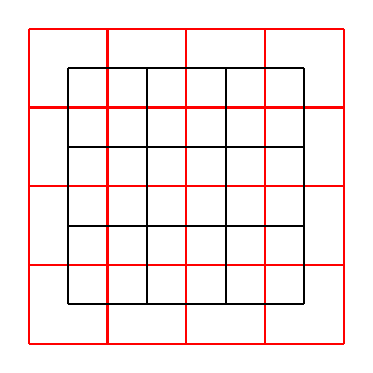
\begin{tikzpicture}
        \draw[step=1.0,thick,red] (0,0) grid (4,4);
        \draw[step=1.0,black,thick,shift={(0.5,0.5)}] (0,0) grid (3,3);
    \end{tikzpicture}
    \caption{The slots for generating a $3\times3$ tile world.}
    \label{fig:tiles-and-slots}
\end{center}

One example of such module is shown in figure~\ref{fig:wfc-module}.
Each module constrains the 8 adjacent slots.
An edge type is specified for each edge, and modules which share an edge must have the same edge type.
For each corner of the module, several tile constraints are specified.
The modules that share a tile must agree on the tile's properties: its height, slant direction (if any) and surface type.
Terrain types can have multiple surface types, each with a different set of modules and a few modules that allow to transition between them.
For example, a \emph{shore} module could have \emph{ground} tiles on one side and \emph{water} tiles on the other.
Some surface types block paths and buildings and some edge types block paths.
What modules are available for the generator will be determined by the terrain type that was chosen for this world.

\begin{center}
    \captionsetup{type=figure}
    \begin{minipage}{.5\textwidth}
        \centering
        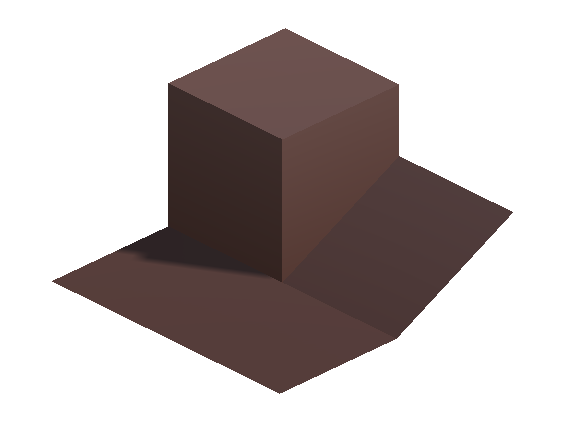
\includegraphics[width=0.95\textwidth]{img/Module model.png}
        \subcaption{The 3D geometry of the module.}
    \end{minipage}%
    \begin{minipage}{.5\textwidth}
        \centering
        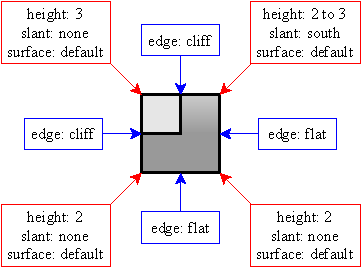
\includegraphics[width=0.95\textwidth]{img/Module constraints.pdf}
        \subcaption{A view from above with the constraints.}
    \end{minipage}
    \caption{An example module and its constraints.}
    \label{fig:wfc-module}
\end{center}

In figure~\ref{fig:wfc-modules}, we show 7 modules as an input.
However, when designing them, it would make more sense to think of them as 3 different modules that can each be rotated.
Thus, the modules we use will also have an option to select the allowed reflection and rotations.
Then, before generating the terrain, we will automatically generate all variants of each module.
Each module can also be placed at different height levels, which is handled similarly.
For example, the module shown in figure~\ref{fig:wfc-module} will effectively become 24 different modules in a terrain type with 4 height levels (0, 1, 2, 3), because it has 8 different reflections and rotations, and it can appear at 3 different height levels (0--1, 1--2, 2--3).

For each module, we also specify a weight.
This dictates how likely it is to be selected when collapsing a slot, compared to other modules.
For example, when we collapse a slot that only has two valid modules, with weights 1 and 4, then the first module will be selected with a 20\,\% probability.

\head{Backtracking}{}
We have decided to implement backtracking to solve contradictions.
If the algorithm only ever has to backtrack once before collapsing another slot, we say that it needs backtracking depth 1.
However, it is possible that the algorithm collapses a slot, finds a contradiction, and after backtracking, removes the only remaining module in the slot that was collapsed.
Thus, it creates another contradiction, which causes it to backtrack deeper.

We ran some quick tests with the set of modules which is going to be used to generate terrain in the demo version.
The results are shown in table~\ref{tab:wfc-backtracking}.
For each test, we tried generating 2000 random worlds, each with three path starts with lengths 24, 28 and 33, making them pretty constrained.

\begin{table}[H]
    \centering
    \begin{tabular}{lrrD{.}{.}{-1}r}
        \toprule
        \textbf{Maximum}            &                          &                              & \mc{}                                &                             \\
        \textbf{backtracking depth} & \halfrow{\textbf{Fails}} & \halfrow{\textbf{Successes}} & \mc{\halfrow{\textbf{Success rate}}} & \halfrow{\textbf{Time (s)}} \\
        \midrule
        0                           & 2000                     & 0                            & 100.00\,\%                           & 644                         \\
        1                           & 786                      & 1214                         & 60.70\,\%                            & 740                         \\
        2                           & 783                      & 1217                         & 60.85\,\%                            & 797                         \\
        10                          & 783                      & 1217                         & 60.85\,\%                            & 819                         \\
        \bottomrule
    \end{tabular}
    \caption{Success rate of terrain generation based on maximum backtracking depth. }
    \label{tab:wfc-backtracking}
\end{table}

No world was able to generate without running into a contradiction, i.e., with a backtracking depth 0.
60.7\,\% of the worlds only ever needed backtracking depth of 1 to successfully generate.
Greater backtracking depth doesn't seem to help very much.
Instead, it makes the generator spend more time trying to save worlds which are still going to fail.
We decided to allow for backtracking depth 1 and otherwise just restart the generation to try again.

\head{Deciding Which Slot to Collapse}{}
We also need to decide which slot to collapse at each step of the algorithm.
Merrell uses in their thesis~\cite{ModelSynthesis} a scan line order, collapsing slots in the lexicographic order of their coordinates.
Gumin in their implementation~\cite{WFC} always collapses a slot with the lowest \emph{Shannon entropy}.
This causes the generation to collapse slots outwards form the slot that was collapsed first.
From our testing, the results tend to look unnatural, often creating regions at the same height, or repeating patterns.

Both approaches grow the collapsed portion of the world from one initial slot, similar to growing a single crystal solid from one seed crystal.
To make the results more natural, we chose to select the slot to collapse at random.
This leads to the generator first collapsing slots in various parts of the world to different configurations.
Then it has to somehow connect these to make the world follow the rules we set.
This leads to much more diverse results, however, the success rate becomes very low, leading to slower generation.

As a compromise, we tried to still select the slots randomly, but give slots with lower entropy a greater weight, so they are more likely to be selected.
Specifically, the weight of each slot is $1/entropy$, making it more likely to select more constrained slots, but still collapsing unconstrained slots once in a while.
This leads to results similar to the ones with uniform randomness, but it increases the success rate.
However, this results in the algorithm being even slower, probably because calculating the entropy of a slot is not trivial.

To remedy this, we tried weighting the slots by the number of invalid slots\,$+\,1$ (the $+1$ at is there to make all weights non-zero).
This is an approximation of the previous metric, still assigning greater weight to more constrained slots.
From our testing, the resulting worlds look still as good as before, but this metric is trivial to compute, so the worlds generate slightly faster.

The tests we ran are summarized in table~\ref{tab:wfc-collapsing}.
For each method, we generated worlds until we successfully generated 1000 of them.
This is to compare the average time it takes to successfully generate a world, which is a more useful metric for us.

\begin{table}[H]
    \centering
    \begin{tabular}{lrrD{.}{.}{-1}r}
        \toprule
        \textbf{Which slot}         &                          &                              & \mc{}                                &                             \\
        \textbf{to collapse?}       & \halfrow{\textbf{Fails}} & \halfrow{\textbf{Successes}} & \mc{\halfrow{\textbf{Success rate}}} & \halfrow{\textbf{Time (s)}} \\
        \midrule
        minimum entropy             & 213                      & 1000                         & 82.44\,\%                            & 492                         \\
        uniformly random            & 823                      & 1000                         & 54.85\,\%                            & 691                         \\
        weighted by $1/$entropy     & 672                      & 1000                         & 59.81\,\%                            & 728                         \\
        weighted by invalid modules & 676                      & 1000                         & 59.67\,\%                            & 656                         \\
        \bottomrule
    \end{tabular}
    \caption{Success rate of terrain generation based on how the algorithm decides which slot to collapse next. }
    \label{tab:wfc-collapsing}
\end{table}

In the end, we chose to select slots to collapse randomly, weighted by the number of invalid modules.
This method is the fastest of the methods that produce worlds that look random.
In figure~\ref{fig:generated-terrain}, we show an example of terrain that was generated this way.

\begin{center}
    \captionsetup{type=figure}
    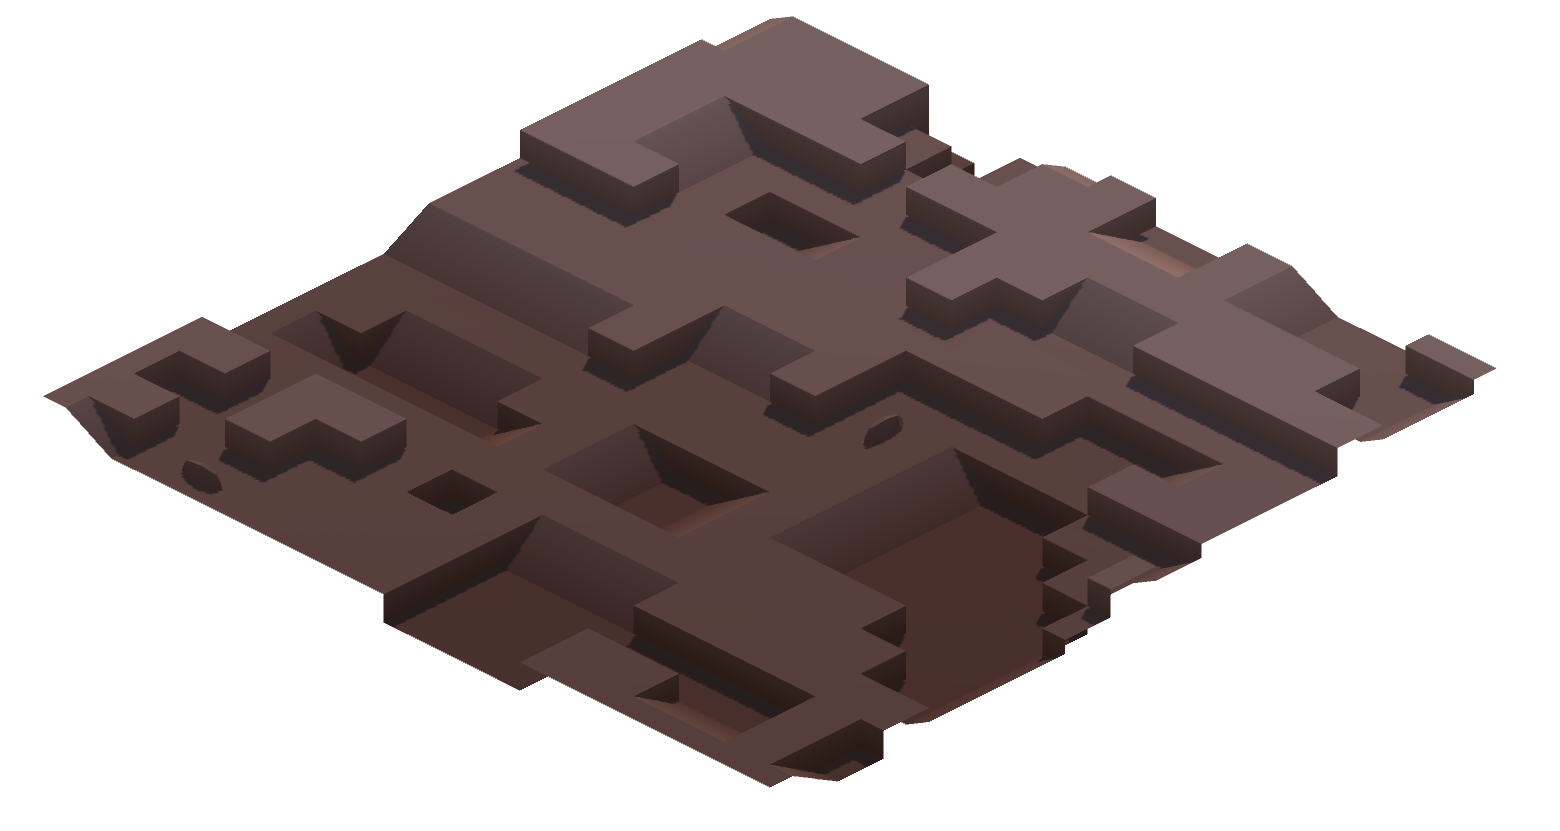
\includegraphics[width=0.85\textwidth]{img/Generated Terrain.png}
    \caption{An example terrain generated using WFC.}
    \label{fig:generated-terrain}
\end{center}

\section{Obstacle Generation}\label{sec:analysis-obstacles}

Now that we have generated the attacker paths and terrain, the next step is to generate obstacles.
We know from section~\ref{sec:design-world}, that each tile can have up to one obstacle placed on it.
They block the tiles, so they cannot appear on path tiles.
Which obstacles can appear, and their placement is controlled by the terrain type.
Before we select an algorithm to place them, we should formalize the parameters which influence the obstacle placement.

\subsection{Obstacle Placement Parameters}

In section~\ref{sec:design-world}, we also specified that some obstacles will be more common than others.
In the terrain type specification, we can assign each obstacle a probability of it appearing on each tile.
Some obstacles, for example the \emph{mineral-rich} and \emph{fuel-rich} ones will also have a maximum and minimum count.

Some obstacles will appear more often or less often around other obstacles.
This means that an obstacle's probability to be placed on a given tile will be influenced by the obstacles already placed on surrounding tiles.
For each obstacle type, the terrain type can specify its \emph{affinity} for each other obstacle type.
When trying to place the obstacle on a given tile, its placement probability will be modified for each already placed obstacle by the affinity for that obstacle times the \emph{closeness} to it.
The closeness is some function that decreases with distance, similar to the \emph{crowding penalty} we used in section~\ref{sec:analysis-our-simulated-annealing} when generating paths.

Since each tile can only have one obstacle, the more important obstacles should be placed before others.
For example, we want the resource providing obstacles to be placed first.
So, the obstacle types will be divided into phases, and the first phase will be placed first, then the second, and so on.

In section~\ref{sec:analysis-our-wfc}, we mentioned that each tile will have a surface type from the set of surface types the terrain type allows.
We also want to limit on which surfaces can each obstacle appear.
For example, we don't want trees to appear in water.
This should be all we need to procedurally place obstacles how we want.

\subsection{Obstacle Placement Algorithm}

Placing the obstacles should be fairly straightforward given the parameters we decided on.
The algorithm should place them phase by phase.
For each phase, it will loop through all tiles, and for each tile, it will assign an obstacle to it with the probability that is calculated for that obstacle for that tile.
The probability is 0 for invalid placements, like path tiles, tiles with another obstacle, or tiles with the wrong surface.
When multiple obstacles from the same phase want to be placed on the same tile, we just select one of them at random.

However, we also have a minimum and maximum count for some obstacles.
To adhere to the maximum count, we can just stop placing the obstacle once the maximum count is reached.
This creates a small problem.
If the algorithm went through the tiles in some predefined order, the tiles at the start would have a higher chance of containing obstacles with a count limit than the tiles at the end.
Because once the algorithm reaches the maximum count, it stops placing them.
We can fix this by enumerating the tiles in a random order.

Enforcing the minimum count is also not difficult.
If we finish a phase and there is not enough obstacles of some types, we can do another placement phase, this time only with the obstacle types which didn't reach their minimum yet.
Assuming there is enough tiles with non-zero probability, we can repeat this process until the right amount obstacles is placed.

This is summarized as algorithm~\ref{alg:obstacle-placement}.
Here, a phase is just a set of obstacle types.
Here, the function \textsc{GetPlacementProbability} also checks if the placement would be valid.
If not, it returns 0.

Of course, there are some optimizations we can make.
For example, we don't have to go through all tiles, only those that don't have an obstacle and don't have a path going through them.

\begin{algorithm}[H]
    \caption{Obstacle placement}
    \label{alg:obstacle-placement}
    \begin{algorithmic}[1]
        \ForEach{phase $p$}
        \While{$p$ is not empty}
        \Statex
        \ForEach{tile $t$ in random order}
        \State $candidates \gets \varnothing$
        \ForEach{obstacle type $o$ in $p$}
        \State $q \gets$ \Call{GetPlacementProbability}{$o, t$}
        \State with probability $q$: $candidates \gets candidates + o$
        \EndFor
        \Statex
        \If{$candidates$ is not empty}
        \State $selected \gets$ random obstacle type from $candidates$
        \State \Call{Place}{$selected, t$}
        \EndIf
        \EndFor
        \Statex
        \ForEach{obstacle type $o$ in $p$}
        \If{number of placed obstacles of type $o \geq o.minimum$}
        \State $p \gets p - o$
        \EndIf
        \EndFor
        \Statex
        \EndWhile
        \EndFor
        \Statex
    \end{algorithmic}
\end{algorithm}

\subsection{Generating Obstacle Models}\label{sec:analysis-obstacle-models}

We can now determine which tiles are blocked by which obstacles.
But by requirement~RW\ref{RW:obstacle-models}, \enquote{each tile with an obstacle will usually contain a whole procedurally generated cluster of obstacle models}.
How do we generate these models?

For any given obstacle type, we can through all the tiles with that obstacle type and place some number of the corresponding model at random points within the tile.
We can also slightly randomize the rotation and scale of the models to achieve a more natural look.
The terrain type then specifies the number of models per tile and the scale and rotation range.

Just placing the models at random points often creates clusters of intersecting models that don't look nice.
So, we let the terrain type set some minimum distance the models should keep from each other.
If it would place a model at a position that's too close to an already placed model, it doesn't place it.

However, this still doesn't feel very natural because the models create squares with hard edges, as shown in figure~\ref{fig:analysis-obstacles-unnatural-boundary}.
We would like the boundaries to be more natural, and even make the models smaller and more spread out near the edges of the boundary.
This is illustrated in figure~\ref{fig:analysis-obstacles-natural-boundary}.

\begin{center}
    \captionsetup{type=figure}
    \begin{minipage}{.5\textwidth}
        \centering
        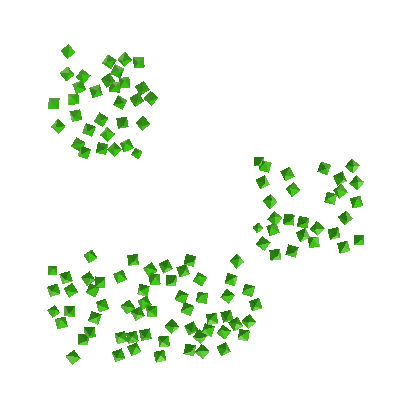
\includegraphics[width=0.95\textwidth]{img/inorganic minerals.png}
        \subcaption{Undesirable result with hard edges.\\\ }
        \label{fig:analysis-obstacles-unnatural-boundary}
    \end{minipage}%
    \begin{minipage}{.5\textwidth}
        \centering
        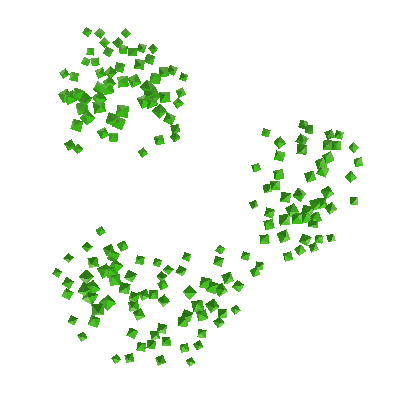
\includegraphics[width=0.95\textwidth]{img/organic minerals.png}
        \subcaption{More desirable result with smooth boundaries.}
        \label{fig:analysis-obstacles-natural-boundary}
    \end{minipage}
    \caption{Comparison of generated obstacle models.}
\end{center}

To place the models in a more natural fashion, we can use what the developers of the game \emph{Factorio}~\cite{Factorio} call \emph{noise expressions}.
Earendel has written a great overview of noise expressions on their blog~\cite{NoiseExpressions}.
The main idea is that we create a function that assigns a numeric value to each point in our world.
For our use-case, the value represents \enquote{how much of an obstacle} is at any given point.
We can then place the obstacle models only where the value is above some threshold, and we scale the models and their spacing by the value too.

We will specify a noise expression for each model in the terrain type.
To do so, we will build up each noise expression from some basic functions, combined using arithmetic operations.
First, we explain the basic functions we will use, and then we'll show how to combine them into a noise expression that is useful for us.
In our examples, we will give each of the basic functions a pseudocode alias to let us express the operations on them better.

\head{Height Function}{}
A simple basic function we might want is a height function.
This function simply tells us what is the height of the terrain at any given point.
The output of this function is shown in figure~\ref{fig:height-fn}.
This function can be useful for example when we want some model to appear only above some specific height.
We denote this function in pseudocode as \mono{height()}.

\head{Signed Distance Functions}{}
The most important basic function is the one that tells us which tiles have on them the obstacle we care about.
After all, we want to place the models on tiles with the obstacle.
We could make a basic function that returns 1 for points within the tiles with the obstacle and 0 otherwise.
However, this doesn't help us make smooth transitions, because we cannot distinguish points that are just outside a tile with the obstacle from points that are far away.
Similarly, we would also like to know how far inside the tile with the obstacle is any given point.
So, we need a \emph{signed distance function}, or \emph{SDF}, a function which tells the distance to a boundary of some region, but is positive inside the region and negative outside.

We will express this function in pseudocode as \mono{obstacle()}.
For greater convenience, we will also specify the scale of the values the function outputs separately for the values inside the region and outside the region.
We will denote these parameters in the pseudocode as \mono{in} and \mono{out}.
In figure~\ref{fig:obstacle-sdf}, we can see an example of this SDF.
The function takes on positive values on the tiles with the obstacle and negative values otherwise, as specified by the parameters.

We can use SDFs to also express the distance to other tiles that are somehow special.
For example the tiles with a path going through them.
We will denote this function as \mono{path}.
An example of this function is shown in figure~\ref{fig:path-sdf}.

\begin{center}
    \captionsetup{type=figure}
    \begin{minipage}{.07\textwidth}
        \centering
        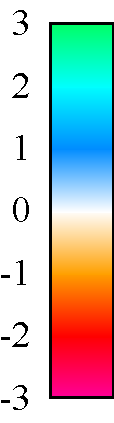
\includegraphics[width=0.95\textwidth]{img/noise expr gradient.pdf}
        \small{\ \\\ \\\ }
    \end{minipage}%
    \begin{minipage}{.31\textwidth}
        \centering
        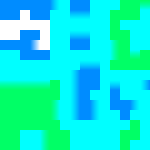
\includegraphics[width=0.95\textwidth]{img/heights.png}
        \small{\mono{height()}}
        \subcaption{Height function.}
        \label{fig:height-fn}
    \end{minipage}%
    \begin{minipage}{.31\textwidth}
        \centering
        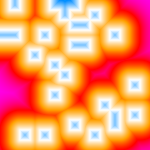
\includegraphics[width=0.95\textwidth]{img/obstacle sdf.png}
        \small{\mono{obstacle(in:1, out:-1)}}
        \subcaption{Obstacle SDF.}
        \label{fig:obstacle-sdf}
    \end{minipage}%
    \begin{minipage}{.31\textwidth}
        \centering
        
\includegraphics[width=0.95\textwidth]{img/path sdf.png}
        \small{\mono{path(in:1, out:-1)}}
        \subcaption{Path SDF.}
        \label{fig:path-sdf}
    \end{minipage}
    \caption{The values of the height function and signed distance functions.}
    \label{fig:basic-fns}
\end{center}

\head{Noise Functions}{}
The basic functions we defined so far are useful, but they still don't let us create shapes without straight boundaries.
For that we can use a noise function.
However, we don't want a function that just gives us some random value for each point, we need the noise to be smooth and change its value gradually as we move in space.
For example \emph{Perlin noise}, developed by Perlin and used in their paper \citetitle{PerlinNoise}~\cite{PerlinNoise}.
It is easy for us to use this function, since it is included in the Unity engine.

In figure~\ref{fig:noise-funcs}, we show what values it produces.
We denote it with the alias \mono{noise}, and it can be scaled up or down to get larger or smaller features using the \mono{scale} parameter.
With a large scale, it might seem too smooth and artificial, while with a smaller scale, the values fluctuate too much.
To solve this, we can use arithmetic to combine the values of multiple noise functions.
By adding together more layers of the noise, each with a different scale and amplitude, we can create a result that has details but doesn't look as random.

\begin{center}
    \captionsetup{type=figure}
    \begin{minipage}{.07\textwidth}
        \centering
        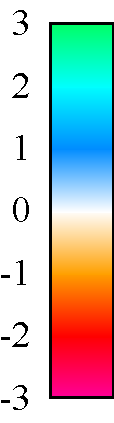
\includegraphics[width=0.95\textwidth]{img/noise expr gradient.pdf}
        \small{\ \\\ \\\ \\\ }
    \end{minipage}%
    \begin{minipage}{.31\textwidth}
        \centering
        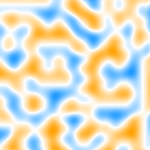
\includegraphics[width=0.95\textwidth]{img/noise2.png}
        \small{\mono{noise(scale:2)\\\ \\\ }}
    \end{minipage}%
    \begin{minipage}{.31\textwidth}
        \centering
        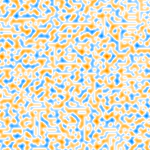
\includegraphics[width=0.95\textwidth]{img/noise3.png}
        \small{\mono{noise(scale:0.5)\\\ \\\ }}
    \end{minipage}%
    \begin{minipage}{.31\textwidth}
        \centering
        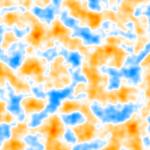
\includegraphics[width=0.95\textwidth]{img/fractal noise.png}
        \small{\mono{noise(scale:2) +\\0.5 noise(scale:1) +\\0.25 noise(scale:0.5)}}
    \end{minipage}
    \caption{Examples of Perlin noise.}
    \label{fig:noise-funcs}
\end{center}

\head{Putting it All Together}{}
In figure~\ref{fig:noise-expr-steps}, we show how we can build up a noise expression that we could use to place obstacle models.
In addition to the basic functions and arithmetic operations, we also use a function called \mono{clamp} which clamps a value between the specified minimum and maximum.
We do this in three steps to show how the output of the noise expression changes with each addition.
Each sub-figure represents one step, and later steps reference the noise expressions from the previous steps in their pseudocode, written as \mono{STEP\_\#}.

\begin{center}
    \captionsetup{type=figure}
    \begin{minipage}{.07\textwidth}
        \centering
        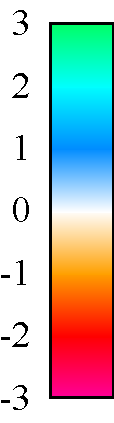
\includegraphics[width=0.95\textwidth]{img/noise expr gradient.pdf}
        \small{\ \\\ \\\ \\\ }
    \end{minipage}%
    \begin{minipage}{.31\textwidth}
        \centering
        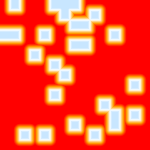
\includegraphics[width=0.95\textwidth]{img/noise expr step1.png}
        \small{\mono{STEP\_1 =\\clamp(min:-2, max:0.2,\\obstacle(in:1,out:-3))}}
    \end{minipage}%
    \begin{minipage}{.31\textwidth}
        \centering
        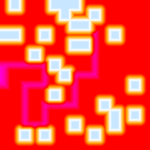
\includegraphics[width=0.95\textwidth]{img/noise expr step2.png}
        \small{\mono{STEP\_2 =\\STEP\_1 +\\path(in:-2, out:0)}}
    \end{minipage}%
    \begin{minipage}{.31\textwidth}
        \centering
        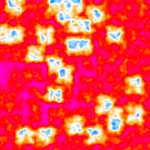
\includegraphics[width=0.95\textwidth]{img/noise expr step3.png}
        \small{\mono{STEP\_2 +\\0.8 noise(scale:0.9) +\\0.54 noise(scale:0.45)}}
    \end{minipage}
    \caption{Building up a noise expression step by step.}
    \label{fig:noise-expr-steps}
\end{center}

When placing the models, we sample many points on each tile and place the model only if the value of the specified noise expression is for that point above some threshold.
The value also determines how close together can the models be and how large they should be.
This lets us be more expressive with model placement and create more natural-looking worlds.
Using the noise expression from figure~\ref{fig:noise-expr-steps}, we have generated the models shown in figure~\ref{fig:analysis-obstacles-natural-boundary}.

\section{Attacker Wave Generation}\label{sec:analysis-waves}

Now that world generation is done, attacker waves are the last remaining part of battles we want to procedurally generate.
In section~\ref{sec:design-attacker-waves} we have outlined that each wave will be composed of batches, and each batch will contain potentially different attackers spawning on each path.
However, the spacing and count will be shared by the whole batch.
We also mentioned, that the waves need to scale in difficulty, ideally slightly faster than the player could realistically handle.
In section~\ref{sec:analysis-procedural-generation} we also decided that this difficulty will be controlled by the map generator.

Our goal in this section will be to create an algorithm for generating these waves, such that their difficulty somewhat matches the requested difficulty.
We were able to find some relevant sources about procedural wave generation in tower defense games, but they generate waves dynamically to adapt to the player's skill, or to find weaknesses in their defenses.
For example, in the paper~\citetitle{NeatWaves}~\cite{NeatWaves}, its authors train a neural network to decide the composition of a wave based on the player's defenses, with the goal to increase engagement.
However, we want the waves to be only based on the requested difficulty.
And, as stated in section~\ref{sec:design-attacker-waves}, we let the player see them in advance, so the player is the one who adapts, not the waves.

There are also some already existing implementations.
For example, even though the waves in the main game modes of \emph{Bloons TD6} are always the same, there are also game modes with randomized waves.
However, the nature of the algorithm used to generate these waves is not publicly known, and it probably wouldn't be useful us, because the generated waves vary in difficulty a lot.
We were unable to find an example of a tower defense game with procedurally generated waves with a consistent difficulty.

To create a good algorithm that generates waves with a specific difficulty, we need to somehow quantify the difficulty of a wave first.
In the following subsections we aim to find a way to express the difficulty of a wave, that is as simple as possible, but it is close enough for the waves to not feel unfair.
It is important to stress that depending on the player's defenses, some waves will be always harder for them to deal with and others will be easier.
However, if a player is unable to beat some wave, we want them to feel like there were ways to prevent this.
In other words, that the wave was beatable, they just didn't play the best way they could.

As we discussed in section~\ref{sec:analysis-procedural-generation}, the world on which the battle takes place greatly influences the difficulty.
However, we will eliminate this variable and try to quantify the wave difficulty in vacuum.
It will be the responsibility of the map generator to select the right wave difficulty based on the parameters it selected for the world.

Let's simplify our problem to as much as we can to make it easy to find an exact solution.
Then we'll gradually add more complications until we get an approximation of the real problem that is good enough.

\subsection{Model 1: Single Attacker}\label{sec:analysis-waves-single}
For our simplest model, we assume that a wave contains only one attacker with some amount of HP, denoted as $h$, and a speed $s$ in tiles per second.
The attacker has no other qualities or special abilities.
We say the player's defense beats this wave when the attacker is killed before it reaches the Hub.

We also imagine each defensive tower $t$ to always deal some fixed amount of damage $d_t$ per second to the first attacker in its range which covers some region of the path that is $l_t$ long.
This means that the attacker will spend $l_t / s$ seconds in its range, taking $d_t \cdot l_t / s$ damage in total.

A defense $T$ that consists of multiple towers can then deal damage equal to the sum of the individual towers.
This means that the defense can beat the wave if and only if the following inequality holds:
\begin{equation}
    \sum_{t \in T} d_t l_t / s \geq h
\end{equation}
We will refer to the total damage the towers would deal to an attacker with speed 1 as \emph{damage capacity} $C$.
It can be calculated as follows:
\begin{equation}\label{eqn:C}
    C = \sum_{t \in T} d_t l_t
\end{equation}
This lets us write the condition more concisely as $C \geq hs$.

From this equation we can see, that the difficulty of this wave is exactly proportional to $hs$.
The defenses that can beat an attacker with 10\,HP and speed~1 are exactly the same as those that can beat an attacker with 5\,HP and speed~2.

This is a great result, but our waves can contain more attackers than one, so we have to generalize.
Next, we will take a look at a case with an infinite amount of attackers.

\subsection{Model 2: Infinite Waves}
For this model, everything is the same as in the previous model, but each wave consists of infinitely many attackers of one attacker type.
We will denote the spacing (or gap) between the attackers as $g$, measured in seconds.
Here, we say the player's defense beats this wave when no attacker ever reaches the Hub.

The towers still deal damage only to the first attacker.
Imagine the first attacker is killed after it has travelled $p$ tiles.
Assuming at least $g$ seconds have passed, the second attacker has already spawned, and it has traveled $p - sg$ tiles, so the defenses have less time to kill it than they had for the first attacker.
If the towers progressively kill the attackers later and later, eventually, one of them will reach the Hub.
Intuitively, the towers need to be able to kill an attacker every $g$ seconds to beat the wave.

When each attacker spends at least $g$ seconds within the range of each tower, then each tower $t$ deals in total $d_t g$ damage to each attacker.
However, when the spacing is larger, some towers won't be able to deal damage to each attacker for $g$ seconds, but only $l_t / s$ as we determined in the previous model.
So, each tower can only deal $d_t$ damage per second for $\min(l_t / s, g)$ seconds.
So, to each attacker, the towers will deal a total damage amount expressed by the following formula:
\begin{equation}
    \sum_{t \in T} d_t \cdot \min(l_t / s, g)
\end{equation}

It is more useful to think about the damage per second, so let $R$ be the total damage per second the player's defenses can deal to the attackers, or the \emph{damage~rate}.
One attacker spawns each $g$ seconds, so we can calculate the damage rate by dividing the previous formula by $g$:
\begin{equation}\label{eqn:R}
    R = \sum_{t \in T} d_t \cdot \min(l_t / (s g), 1)
\end{equation}
We see that $R$ is at most $\sum_{t \in T} d_t$, and it is equal to it only when $l_t / (s g) \geq 1$ for each tower $t$.

$R$ is also at most $\sum_{t \in T} d_t \cdot l_t / (s g)$, and it is equal to it in the other cases.
Since $s$ and $g$ are not dependent on the tower $t$, we can bring them in from of the sum:
\begin{equation}
    \frac{1}{s g} \sum_{t \in T} d_t \cdot l_t / (s g)
\end{equation}
This sum is by definition equal to $C$ (see equation~\ref{eqn:C}), so we can substitute to get the following relation between $R$ and $C$:
\begin{equation}\label{eqn:RC}
    R \leq \frac{C}{s g}
\end{equation}

Since one attacker spawns every $g$ seconds, the towers can deal at most $Rg$ damage to each attacker.
Each attacker has $h$\,HP, so the player will beat the wave if and only if $Rg \geq h$.

As described before, sometimes $R$ does not depend only on the player's defenses, but also on the attacker speed $s$ and spacing $g$.
However, this should be very rare, because the maximum spacing we will use is $g=2$ seconds, and no attacker will be faster than $s=4$ tiles per second, which is still extremely fast compared to most attackers.
This means that every tower has to have $l_t \geq 8$ for $g$ and $s$ to never influence $R$, which is easily achievable with most tower types.
For now, we can think of $R$ as being a constant determined by the player's defenses.

\subsection{Model 3: Finite Waves}\label{sec:analysis-waves-finite}
In this model, we add another parameter to our wave.
The wave is once again composed of attackers with $h$ HP and speed $s$, coming with a spacing of $g$ seconds, but this time, there is exactly $n$ of them.
How do we judge the wave difficulty now?

The best way to think about this is that the player's towers need to deal $nh$ damage in total.
From \hyperref[sec:analysis-waves-single]{model~1} we know that if the whole wave was a single attacker, the player's defenses would deal $C/s$ damage in total.
So, they would defeat the wave if and only if $C/s \geq nh$.

The towers still target only the first attacker, so they will kill it first.
Then, they can deal with the second attacker, but the second attacker is $g$ seconds behind the first, so they have $g$ more seconds to deal with it.
This is also true for each other attacker, so the towers effectively get $g$ seconds of firing for free for each attacker beyond the first.
Thus, a more accurate condition for beating the wave is the following inequality:
\begin{equation}
    C/s + (n-1) R g \geq nh
\end{equation}
When we put all wave-dependent terms on the right and rearrange, we get that the player beats the wave if and only if the following condition is satisfied:
\begin{equation}\label{eqn:beat-finite-wave}
    C \geq s(nh - (n - 1)Rg)
\end{equation}

We cannot quantify the difficulty of the wave with one number anymore.
For example, there exists a defense $T_1$ which beats the wave, and another defense $T_2$ which also beats it despite having lower $C$, because it has greater $R$.
So, we have to accept that each defense has two characteristic values.

We aim to illustrate how the required damage capacity and rate change based on the wave parameters using figure~\ref{fig:model3}.
The blue area represents the defenses which can beat the wave, and the white area represents those which can't.
The orange area shows defenses that can't exist because they would violate inequality~\ref{eqn:RC}.
We also highlight two points in each plot, each of these points represents one example defense.
$T_1$ consists of one tower with $d_t=5$ and $l_t=12$.
$T_2$ consists of one tower with $d_t=10$ and $l_t=1.5$ which is an unusually small path coverage.

Figure~\ref{fig:model-3-base} shows a wave which we will use as a base case for our comparison.
We can see that both $T_1$ and $T_2$ are able to beat it.
In figure~\ref{fig:model-3-h20} we can see what happens when the attacker health becomes 20\,HP.
Neither of the defenses are able to beat it now.
Figure~\ref{fig:model-3-s2} shows that increasing the speed $s$ to 2 causes problems for towers with small path coverage $l_t$.
We can see that the damage rate of defense $T_2$ has decreased because each attacker spends less than $g$ seconds in the range of the only tower.

\begin{center}
    \captionsetup{type=figure}
    \begin{minipage}{.33\textwidth}
        \centering
        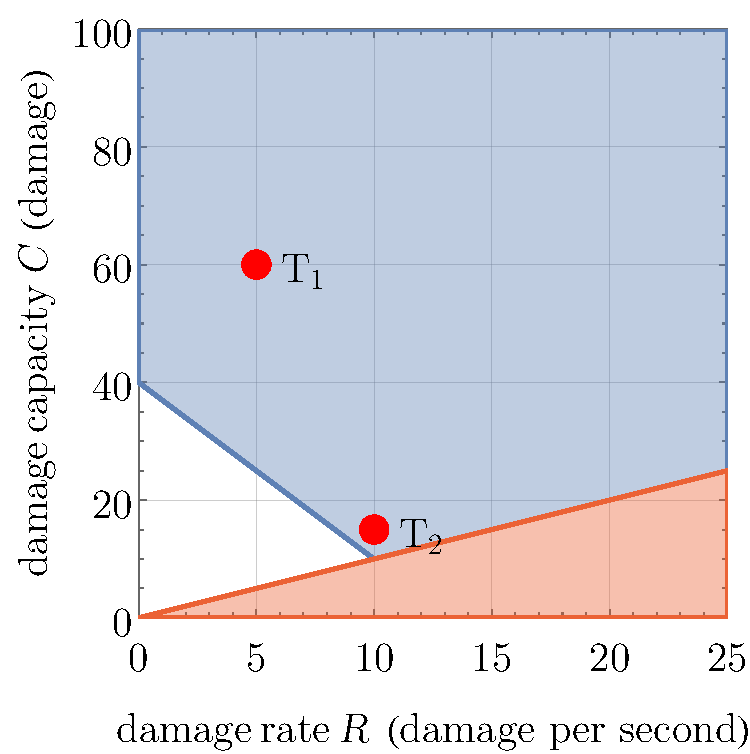
\includegraphics[width=0.95\linewidth]{img/model3 base.pdf}
        \subcaption{$h=10, s=1,$\\$ g=1, n=4$}
        \label{fig:model-3-base}
    \end{minipage}%
    \begin{minipage}{.33\textwidth}
        \centering
        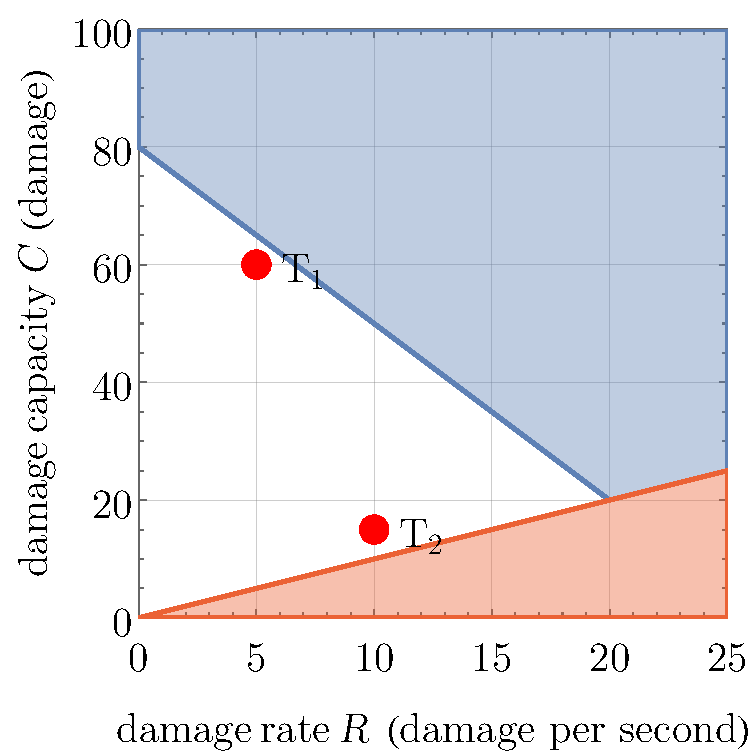
\includegraphics[width=0.95\linewidth]{img/model3 h20.pdf}
        \subcaption{$\bm{h=20}, s=1,$\\$ g=1, n=4$}
        \label{fig:model-3-h20}
    \end{minipage}%
    \begin{minipage}{.33\textwidth}
        \centering
        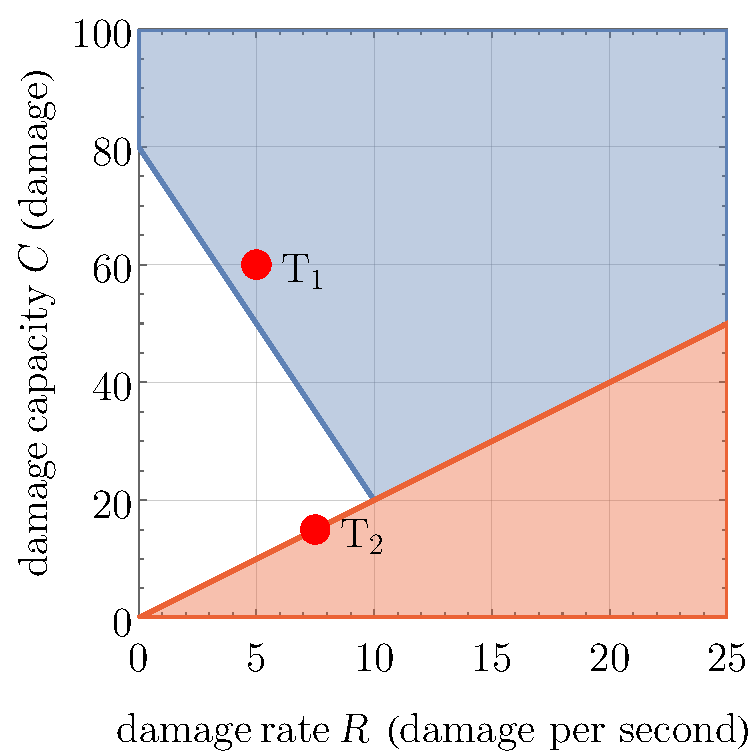
\includegraphics[width=0.95\linewidth]{img/model3 s2.pdf}
        \subcaption{$h=10, \bm{s=2},$\\$ g=1, n=4$}
        \label{fig:model-3-s2}
    \end{minipage}\\
    \begin{minipage}{.33\textwidth}
        \centering
        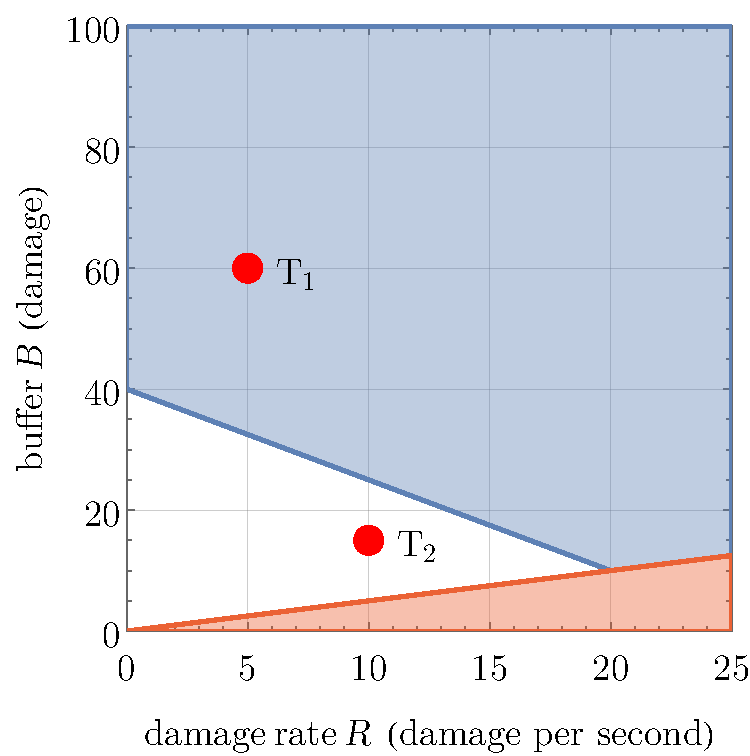
\includegraphics[width=0.95\linewidth]{img/model3 g0.5.pdf}
        \subcaption{$h=10, s=1,$\\$ \bm{g=0.5}, n=4$}
        \label{fig:model-3-g0.5}
    \end{minipage}
    \begin{minipage}{.33\textwidth}
        \centering
        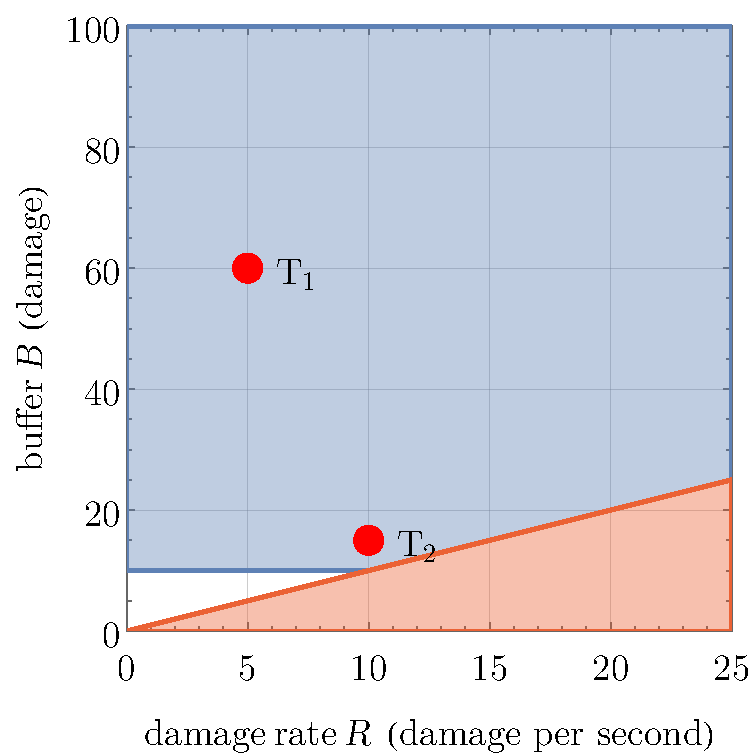
\includegraphics[width=0.95\linewidth]{img/model3 n1.pdf}
        \subcaption{$h=10, s=1,$\\$ g=1, \bm{n=1}$}
        \label{fig:model-3-n1}
    \end{minipage}%
    \begin{minipage}{.33\textwidth}
        \centering
        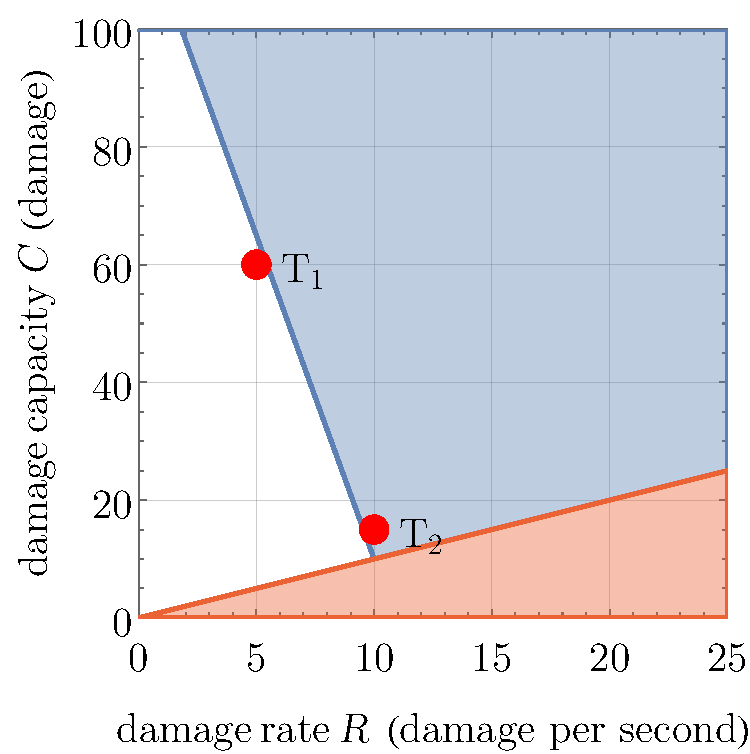
\includegraphics[width=0.95\linewidth]{img/model3 n12.pdf}
        \subcaption{$h=10, s=1,$\\$ g=1, \bm{n=12}$}
        \label{fig:model-3-n12}
    \end{minipage}%
    \caption{Which defenses can beat various attacker waves, according to model 3.}
    \label{fig:model3}
\end{center}

In figure~\ref{fig:model-3-g0.5} we can see that with smaller spacing of $0.5$ seconds between the attackers, damage rate becomes less effective.
A similar effect can be seen when we decrease the number of attackers.
As shown in figure~\ref{fig:model-3-n1}, when the wave contains only one attacker, damage rate is irrelevant.
On the other hand, when there are many attackers, the damage rate becomes much more important than capacity.
In figure~\ref{fig:model-3-n12} we can see $T_1$ cannot beat a wave with 12 attackers, but $T_2$ can.

Thus, we need both parameters $R$ and $C$ to accurately describe which defenses can beat the wave and which cannot.

\subsection{Model 4: Damage in an Area}\label{sec:analysis-waves-aoe}
Many towers will be able to deal damage to all attackers in some area.
These towers are much more effective against large groups of attackers, especially when they are close together.
We can model these towers similarly to what we have done so far, but we will add one more parameter, the damage range $r_t$.
Now, each tower $t$ deals $d_t$ damage per second to the first attacker, but also all the attackers at most $r_t$ tiles behind it.
This still makes all calculations much more difficult, so we will choose to ignore many edge cases.

Intuitively, for the first attacker of every wave, nothing changes.
To kill it, the condition $C/s \geq h$ still holds.
Killing the second attacker is easier as it has already been damaged by collateral damage.
The attackers spawn $g$ seconds apart, so each can travel $sg$ tiles before the next one spawns, making the gaps between them $sg$ tiles long.
So, the second attacker has been receiving collateral damage from all towers $t$ with $r_t \geq sg$.
But how much damage is that?

To simplify our calculations, we will introduce some new variables $R_k$.
$R_1$ is the damage rate (see equation~\ref{eqn:R}) of towers which hit one extra attacker with collateral damage, $R_2$ for towers which deal damage to two extra attackers, and so on.
Formally,
\begin{quotation}
    $\forall k \in \mathbb{N}^+$ let $R_k$ be the damage rate of towers $t$ with $r_t \geq ksg$.
\end{quotation}

Killing the first attacker will take $t_1 = h/R$ seconds as usual, and in the time, the second attacker will take $t_1 R_1$ collateral damage.
In general, the $k$th attacker will take $t_1 R_{k-1}$ collateral damage from towers shooting at the first attacker.
Let $t_k$ be the time it takes for the $k$th attacker to be killed by towers continuously shooting at it.
It is equal to the remaining health the attacker will have after the ones before it have been killed, divided by $R$:
\begin{equation}\label{eqn:time-to-kill}
    t_k = \frac{1}{R}\left(h - \sum_{i=1}^{k-1} t_i R_{k-i} \right)
\end{equation}

This formula isn't useful yet, because we still need too many variables to specify the player's defenses.
However, this calculation can be simplified with the right assumptions.
The game should force the player use towers that deal damage in an area, in addition to those with a single target.
So, when generating the waves, we can just assume the player has these towers.
This in turn makes the player use them in order to beat the wave.

The greater the tower's damage range $r_t$, the less damage it should deal and the less often it should appear.
Let's assume that in a balanced defense, the towers' damage rate decreases exponentially with increasing $r_t$.
\begin{quotation}
    We say that a defense $T$ is $(\alpha, \beta)$\emph{-balanced} for some $\alpha,\beta \in (0,1)$ when $\forall x \in \R^+$ the total damage rate of towers $t \in T$ with $r_t \geq x$ is equal to $\alpha\beta^x R$.
\end{quotation}
We will select the right $\alpha$ and $\beta$ based on playtesting.
Since towers with larger damage range are generally going to be more expensive than single-target towers, we will make these parameters very small at the start of each level, only reaching their intended values after a few waves.

Now we can precisely determine all $R_k$ for a given wave.
From the definition, $R_k$ is the damage rate of towers with $r_t \geq ksg$, so $R_k = \alpha\beta^{ksg} R$.
We can substitute this into equation~\ref{eqn:time-to-kill} to get the following recurrence relation:
\begin{equation}
    t_k = \frac{1}{R}\left(h - \sum_{i=1}^{k-1} t_i \alpha\beta^{(k-i)sg} R\right)
\end{equation}
We can calculate its closed-form solution\footnote{To calculate this, we first transformed the recurrence into one that depends only on the previous term, and then we used \emph{Wolfram Mathematica}~\cite{Mathematica} to calculate the closed-form solution.}:
\begin{equation}
    t_k = \frac{h}{R}\left(\frac{
            1-\alpha-\beta^{sg}+\alpha\beta^{sg}+\alpha(1-\alpha)^k\beta^{sgk}
        }{
            (1-\alpha)(1-\beta^{sg}+\alpha\beta^{sg})
        }\right)
\end{equation}

Now we can finally construct an updated condition for beating this wave.
By definition of $t_k$, we know that each attacker will have $Rt_k$ HP when all attackers before it die.
So, the player's defenses needs to deal in total $\sum_{k=1}^{n} Rt_k$ damage to all the attackers while they are the first attacker alive, instead of $hs$.
Otherwise, the derivation is the same as for \hyperref[sec:analysis-waves-finite]{model~3}, so the player will beat a wave if the following inequality holds:
\begin{equation}
    C/s + (n-1)Rg \geq \sum_{k=1}^{n} Rt_k
\end{equation}
If we put all wave-dependent terms on the right side of the equation and rearrange, we get the following inequality:
\begin{equation}
    C \geq s\left(Rt_1 + \sum_{k=2}^{n} (Rt_k - Rg)\right)
\end{equation}

However, there is still one problem we overlooked.
We are using $Rg$ as the extra damage each attacker beyond the first will take, because it is $g$ seconds behind the attacker before it.
However, this damage can never be greater than the attacker's health, $Rt_k$ in this case.
This wasn't a problem in \hyperref[sec:analysis-waves-finite]{model~3}, because this would only happen in waves the player would beat anyway.
So, we get the following updated condition:
\begin{equation}
    C \geq s\left(Rt_1 + \sum_{k=2}^{n} \max(Rt_k - Rg, 0)\right)
\end{equation}

If we substitute the definition of $t_k$, we get the following inequality:
\begin{equation}
    C \geq s\left(h + \sum_{k=2}^{n} \max \left(
        h\frac{
                1-\alpha-\beta^{sg}+\alpha\beta^{sg}+\alpha(1-\alpha)^k\beta^{sgk}
            }{
                (1-\alpha)(1-\beta^{sg}+\alpha\beta^{sg})
            }
        - Rg, 0
        \right)\right)
\end{equation}
We would like to get rid of the summation, but this is tricky because of the maximum function.
However, for the parameters we allow, $t_k$ is always decreasing with $k$.
This means that for some $n^*$, the first $n^*$ terms of the summation will be greater than zero and the rest will be zero.
This lets us discard the maximum function and simplify the condition further:
\begin{equation}
    C \geq s\left(h - (n^*-1)Rg + h\sum_{k=2}^{n^*} \frac{
        1-\alpha-\beta^{sg}+\alpha\beta^{sg}+\alpha(1-\alpha)^k\beta^{sgk}
    }{
        (1-\alpha)(1-\beta^{sg}+\alpha\beta^{sg})
    }
    \right)
\end{equation}

Finally, we can calculate the closed-form solution\footnote{\emph{Wolfram Mathematica} was used to find the closed-form solution.} for the summation to obtain that the player's defenses will beat a wave if and only if the following condition is satisfied:
\begin{equation}\label{eqn:beat-model-4}
    C \geq s\left(\frac{
    n^*(\beta^{sg}-1) - \alpha\beta^{sg}((1-\alpha)^{n^*}\beta^{sgn^*} + n^*(\beta^{sg}-1) - 1)
    }{
        (1+(\alpha-1)\beta^{sg})^2
    }h
    - (n^*-1)Rg
    \right)
\end{equation}
Where $n^*$ is the smallest $k$ between 1 and $n$, such that the following inequality holds:
\begin{equation}
    \frac{
        1-\alpha-\beta^{sg}+\alpha\beta^{sg}+\alpha(1-\alpha)^k\beta^{sgk}
    }{
        (1-\alpha)(1-\beta^{sg}+\alpha\beta^{sg})
    } \leq \frac{Rg}{h}
\end{equation}
In case no such $k$ exists, we set $n^*$ to $n$.

\subsection{Model 5: Multiple Batches}
So far we have considered only waves with one attacker type.
In section~\ref{sec:design-attacker-waves} we mentioned that waves can consist of up to three batches.
Each batch contains some number of attackers of the same attacker type, spaced apart by some spacing.
We can specify a set of wave parameters for each batch $b_k$ instead of having one for the wave as a whole.
These parameters have a subscript which denotes which batch they correspond to, for example the first batch ($b_1$) contains $n_1$ attackers with $h_1$\,HP and speed $s_1$, with a gap of $g_1$ seconds between them.

To determine which defenses will beat a wave with $N$ batches, we can extend the condition for \hyperref[sec:analysis-waves-aoe]{model~4}.
We will refer to the right-hand side of inequality~\ref{eqn:beat-model-4} as the total value of the attackers.
For simplicity, we can then denote the total attacker value with the parameters for batch $b_k$ as the batch value $V_k$.
The defenses now have to beat all the batches one by one, but they still have the same damage capacity $C$ to work with.
So, we can say the defenses will beat the wave when the following inequality holds:
\begin{equation}
    C \geq \sum_{k=1}^{N} V_k
\end{equation}

We also specified that the spacing between batches will be 1 second, but the previous condition acts like the next batch begins right as the previous one ends.
So, we need to add 1 additional second of firing to each wave beyond the first.
An updated condition could look like this:
\begin{equation}
    C \geq V_1 +\sum_{k=2}^{N} \max(V_k - s_kR, 0)
\end{equation}
Again, we limit the batches to have a non-negative value, because the towers cannot \enquote{restore the damage capacity} by dealing damage to dead attackers.

Even though they are not visible now, the collateral damage calculations are all wrong.
We never investigated what happens with an uneven attacker spacing, however we don't even know what's the spacing going to be like.
We know how far each attacker spawns behind the attacker before it, but attackers from different batches can have different speeds, so the spacing between them changes as they move, and they can even overtake each other.
There really isn't a way to capture this behavior in our model without making it much more complicated.
So, we will ignore it, and hope that the waves we generate don't deviate in difficulty too much from our estimate.
If this ends up being a problem, we can adjust the wave generation algorithm to only produce waves that aren't problematic.

\subsection{Model 6: Multiple Paths}\label{sec:analysis-waves-paths}
The levels in our game can have multiple paths, and we can even spawn different attackers on each path.
Since all paths in a single level will have similar lengths, we can treat them all the same.
To start, we'll assume that the paths don't interact in any way and that each tower can only shoot at attackers on one path.
This means that each path $p_k$ will have its own damage capacity $C_k$ and rate $R_k$.
The player's defenses then beat a wave if they beat it on each path.

However, when generating a wave, we generate it based on the difficulty determined by the map generator.
We want the difficulty of each path to vary between waves, but the overall difficulty to smoothly increase.
It would be weird for the map generator to dictate the difficulty of each path separately, the wave generator should take care of that.
So, it only specifies the total difficulty using one damage capacity $C$ and rate $R$ and for each wave, the wave generator will divide them between the paths.

\subsection{Model 7: Abilities}\label{sec:analysis-waves-abilities}
So far, we've only considered attackers that have no abilities, towers with no special abilities, and we ignored the abilities the player can use (see section~\ref{sec:design-abilities}).
In this section, we will incorporate these into our wave difficulty estimate.

Usable abilities usually provide one-time damage to the attackers, so they effectively contribute to the damage capacity of the player's defenses.
Similarly, special abilities of towers or other buildings which have some effect on the attackers, usually just make the defense more effective, thus increasing its damage capacity or rate.
These should all be balanced based on playtesting, so they aren't too weak or too strong.
Thus, they don't need any special treatment in our calculations.

On the other hand, attacker abilities is something the wave generator should take into account.
We don't want it to spawn lots of attackers which have very strong abilities just because of their low HP and slow speed.
These abilities can vary widely in their effect and can interact in unpredictable ways.
However, we think it's enough to assign each attacker a value which will be used in all the calculations we did so far instead of their HP.
For example, an attacker with no special abilities and 10\,HP will still have a value of 10.
If it had an ability that makes it take 50\% less physical damage, its value might be about 13.
Also, the damage rate of a defense (see equation~\ref{eqn:R}) is influenced by the attacker speed, but we treated it as a constant the whole time.
We can increase the value of very fast attackers to offset this, treating super-speed as a kind of special ability.
The important thing is that this value can be tweaked based on playtesting.

This way of quantifying the wave difficulty should be good enough to let us produce waves that vary widely in their feel, but are consistent in their difficulty, so they don't feel unfair to the player.

\subsection{Wave Generation Overview}

In the previous sections we decided that the map generator will specify the difficulty of each wave using the value rate and capacity.
Rate basically represents how much damage we expect the player's defenses to deal to an attacker per second.
Capacity basically represents how much damage we expect the defenses to deal to an attacker during its travel from the path start to the Hub.
We derived some formulas which tell us the total attacker value, and we say that a defense can beat a wave if its value capacity is greater than the total attacker value.
Now that we can quantify the difficulty of a wave, we can start generating them.
Our goal for each wave is to generate a random wave, but it has to have a total value very close to the expected capacity without going over.

We also know how many paths are in the level and what attackers we are allowed to use.
In addition to the parameters prescribed by the map generator, the wave generator itself is going to have more parameters which we can tweak based on playtesting, in order to produce the best results.
The first parameters the wave generator will have are limits on the maximum wave length, and the maximum number of attackers, because we don't want waves that are way too long or have way too many attackers.
In section~\ref{sec:analysis-waves-aoe} we also mentioned that the wave generator will have parameters $\alpha$ and $\beta$ that dictate the expected distribution of collateral damage.

In section~\ref{sec:design-attacker-waves} we specified that each wave doesn't have to spawn attackers on every path.
Of course, each wave should always spawn attackers on at least one path.
So, for each wave we will select one path as forced, and each path from the rest will be also selected for this wave with some probability which will be specified as another parameter.

We also decided that there will be two types of waves.
We will call these types \emph{sequential} and \emph{parallel}.
Sequential waves consist of up to three batches of attackers, each with a different attacker type.
Parallel waves consist of only one batch, but they can spawn a different attacker type on every path.
There is no reason to make the first few waves complex, so we limit waves 1 and 2 to just one batch, and waves 3 and 4 to two batches.
Additionally, we will allow each wave to only use the attacker types the waves before it used plus at most one new attacker type.

In section~\ref{sec:analysis-waves-paths} we decided that we will evaluate the value rate, capacity and attacker value separately for each path.
And that it is up to the generator how it will split up the value rate and capacity between the individual paths.
However, that doesn't mean it should be just random.
The towers the player builds are permanent, so each tower contributes its firepower to some paths from the moment its built until the battle ends.
It would be really difficult for the player, if one wave spawned all its attackers on one path, and then another wave expected the player to have as many defenses on another path.
So, we keep track of the expected rate and capacity per path.
For every wave, only the extra rate and capacity it has over the previous wave is to be distributed between the paths freely.

However, the towers can cover multiple paths, and abilities can also be used on any path the player wants.
So, we will reserve a fraction of the capacity as \emph{global}, which can be used by any path and is not locked in afterwards.
How big of a fraction will this be is another parameter to be determined by playtesting.

The generator starts each wave by selecting which paths it will use.
Then the generator randomly picks which wave type this wave will be, with the distribution also specified as a parameter.
Finally, it will generate the random wave, such that a defense with the expected value rate and capacity can beat it.
Any capacity that's left over then gets added to the next wave to compensate.
Since sequential and parallel waves will each be generated with a different algorithm, we will describe them separately in the following subsections.

\subsection{Generating Sequential Waves}

A sequential wave consists of up to three batches of attackers, each with a different attacker type.
We want to select a random number of a random attacker type with a random spacing for each batch, and we are trying to use up as much of the capacity without going over.
Notably, the same attackers will spawn on each of the selected paths.
This means that we also expect the selected paths to have the same rate and capacity.

\head{Distributing new rate and capacity evenly}{}
So, the first thing the algorithm does is distribute the new rate and capacity.
We would like all paths to be equal, but we have to respect the rate and capacity values they have now, and we can distribute only the rate and capacity that are new for this wave.
So, we at least make them as even as possible.
This can be done by always giving to all paths with the lowest amount the amount required to reach the next lowest amount.
Once they are all even, we split evenly the rest.
However, there is no guarantee that the rates and capacities of all paths will be equal.

\head{Rejection sampling}{}
Now we can actually generate the wave.
The most straightforward approach would probably use rejection sampling.
Generate the specified number of completely random batches and check if whether the total value doesn't overshoot the capacity.
If it does, we try again.
To use up the capacity as much as possible, we can generate many waves and select the one which has the greatest total attacker value.
This approach could work, but it has obvious flaws that cause it to produce invalid results very often.
We can improve this by removing them from the options for random selection.

\head{Removing invalid options in advance}{}
For each batch, we first find all the valid attacker types this batch could consist of.
We cannot use an attacker we have already used in a previous batch of this wave, so we filter out those.
Also, if an attacker's value is so great, that spawning only one on each path overshoots the capacity, it is invalid.
When we select a random attacker now, it is guaranteed to be valid.

Another problem a wave might have is that it has simply more than the maximum allowed attacker count, or it might be too long.
It is also possible the wave overshoots the maximum capacity.
So, after picking a random attacker type and a random spacing for a batch, we calculate the maximum number of these attackers the batch can have while staying within these limits.
We then select a random attacker count between 1 and this maximum count.

\head{Ensuring every generated wave uses up the capacity}{}
This guarantees that each wave we generate is valid.
However, we still need to generate many waves to find one that uses up the capacity somewhat well.
To fix this, for the last batch of the wave, we select the spacing and attacker count that minimize the remaining capacity.
This, however, isn't enough to guarantee that every wave we generate is good.
It is possible for the last batch to select an attacker and spacing, such that it's impossible to use up the remaining capacity.
This can happen because with collateral damage, some attackers don't contribute to the total attacker value anymore after some count, as described in section~\ref{sec:analysis-waves-aoe}.
Or simply because the previous batches used up too much of the wave duration or attacker count.

To remedy this, we add another condition when determining the valid attackers for the last batch of the wave.
We remove the attacker types with which we cannot use up the remaining capacity.
However, both the maximum amount of attackers we can use, and their value depends on the spacing we choose.
So we have to check each spacing, and reject the attacker types for which none of the spacings work.
Thus, for the last batch, we don't enumerate only the valid attacker types, but for each we also enumerate all the valid spacings.

This still doesn't ensure the previous waves didn't use up too much of the attacker count or wave duration.
So, if a batch is unable to use up the remaining capacity completely, given the selected attacker type and spacing, we reduce its maximum count by one third, to leave some space for the next batches.
Assuming there is enough different attacker types available, so that we never encounter a situation where there are no valid attackers available, this approach will always produce a valid wave that uses up most of the value capacity.

The whole process of generating a sequential wave is summarized as algorithm~\ref{alg:wave-sequential}.

\begin{algorithm}[H]
    \caption{Generating a sequential wave}
    \label{alg:wave-sequential}
    \begin{algorithmic}[1]
        \State distribute new rate and capacity evenly
        \Statex
        \For{$i$ from 1 to batch count $N$}
        \State find all valid attacker types and spacings
        \State $a \gets$ random valid attacker type
        \Statex
        \If{$i \neq N$}
        \State $s \gets$ random valid spacing for $a$
        \State $max \gets$ calculate maximum attacker count
        \State $c \gets$ random attacker count between 1 and $max$
        \State $b_i \gets (a,s,c)$
        \Statex
        \Else
        \ForEach{valid spacing $s$ for $a$}
        \State $c_s \gets$ calculate maximum attacker count
        \EndFor
        \State $b_i \gets (a; s$ and $c_s$ that maximize total value$)$
        \EndIf
        \EndFor
        \State \textbf{return} $b_1 \dots b_N$
        \Statex
    \end{algorithmic}
\end{algorithm}

\subsection{Generating Parallel Waves}

For generating a parallel wave, we will use a different approach.
A parallel wave consists of only one batch that can spawn different attacker types on every path.
But because it is one batch, all paths have the same number of attackers and the same spacing.
Since we don't yet know the relative difficulty of the attackers we'll spawn on each path, we will keep the new value rate and capacity for this wave unassigned for now, and we will distribute them to the paths only after we have generated the wave.

\head{Comparison to generating a sequential wave}{}
Some requirements are the same as for a sequential wave: the wave cannot be longer than the maximum duration, it cannot have more than the maximum attacker count, and we want to use up as much of the capacity without going over.
We will add some more that naturally extend these:
Since we want to use up most of the capacity, it would make sense to use up all individual path capacities.
We will again use up the global capacity by increasing the number of attackers as much as we can.
To do this effectively, we will want from each path to have enough capacity for at least few attackers on its own.
This allows for more granularity, for example the difference in value between 3 and 4 attackers is smaller than between 1 and 2 attackers, so we can get closer to the capacity limit.

To generate the wave, we first select a random spacing.
Then we want to find a random set of attacker types, one attacker type for each path, such that it produces a valid wave, if we select the maximum amount that doesn't go over the maximum capacity.
Similarly to a sequential wave, we can filter out all the attacker types that are invalid given the selected spacing.
However, this time they can be different for every path.
Based on our requirements, at least some attackers of the type must fit within the current path capacity plus the current global capacity.
This amount will be specified as a parameter based on playtesting.
We also check that it is possible to use up the current path capacity using this attacker type and spacing.

Again, we could select random sets of attackers from these options until we find one that is valid.
However, these validity tests can help us determine which attacker to change in case the set is not valid.
We start by selecting a random attacker for each path from the set of valid attackers for that path.
Then we enter a loop, where we do some tests, and if the set fails one of the tests, we change one attacker type and try again.
If all tests succeed, we then produce the finished wave and distribute the new rate and capacity accordingly.

\head{Using up the path capacities}{}
First, we test that it's possible to use up every path capacity:
We calculate the minimum number of attackers the wave must have in order to use up every path capacity.
We then check if this count is even a viable option for this wave.
Specifically, we check whether this number of attackers would fit within the total capacity, including the new rate and new capacity we still haven't assigned.
To do this, we first calculate the value of the attackers for each path and sum these values together.
We now compare this value to the total combined value of all the capacities, including the new capacity and new rate.
Since we know how many attackers are in the wave, we can convert the new rate to the maximum amount of extra capacity it will provide by multiplying it by the number of attackers after the first.
If the total value of the attackers is greater than the final capacity, it means that we need at least some amount of attackers to fill each path capacity, but this amount would not fit within the final capacity, so this set is not valid.

This usually happens because some attacker had too much value relative to its path's rate and capacity, compared to the other attackers.
So, this is the one attacker will change for another random attacker.
Specifically, we change the attacker type of the path whose value in the previous test overshot its path capacity by the most.
Then we try the test again with this new set.

\head{Using up the global capacity}{}
If the test succeeds, we know the minimum number of attackers the wave can have in order to use up every path capacity.
We also want to ensure this set of attackers can use up most of the capacity, given the constraints on the maximum wave duration and attacker count.
So, as a second test, we calculate the maximum number of attackers these restrictions let us use, and then we check whether the value of this many attackers plus one is more than the total capacity in the same way as in the previous test.
If the value is less than the capacity, it means that the maximum allowed attacker count still doesn't let us use up the capacity as much as we would want.

This time, the issue is that the attackers we want to use don't have enough value to use up the capacity.
So, we change the attacker type of the path whose value in the previous test overshot its path capacity by the least.

\head{Attacker count and distributing new rate and capacity}{}
If both tests succeed, we have found a good enough set of attackers for this wave.
Now we just find the exact maximum number of attackers that will fit within the total capacity, and the wave is finished.
We don't have a formula for this, but we can determine if a specific count fits within the total capacity or not, as we did in the tests.
So, we can find the exact maximum count using binary search.

We have now generated a valid parallel wave, but we still have to somehow distribute the new rate and capacity to the individual paths.
To mimic what the player might do to handle this wave, we calculate by how much the attacker value overshoots the capacity of each path, and we distribute the new rate and capacity in the same proportion.

Again, assuming there is enough different attacker types, this process always produces a valid wave that uses up most of the capacity.
The whole process of generating a parallel wave is summarized as algorithm~\ref{alg:wave-parallel}.

\begin{algorithm}[H]
    \caption{Generating a parallel wave}
    \label{alg:wave-parallel}
    \begin{algorithmic}[1]
        \State select a random spacing $s$
        \State for each path find all valid attacker types
        \State $S \gets$ random valid attacker for each path
        \Statex
        \State $min \gets$ calculate minimum attacker count to use up the all path capacities
        \If{value of $min$ attackers > total capacity}
        \State $p \gets$ path with the greatest value over the path capacity
        \State $S_p \gets$ random valid attacker
        \State \textbf{go to} 4 \Comment{Try again.}
        \EndIf
        \Statex
        \State $max \gets$ calculate maximum attacker count
        \If{value of $max + 1$ attackers < total capacity}
        \State $p \gets$ path with the lowest value over the path capacity
        \State $S_p \gets$ random valid attacker
        \State \textbf{go to} 4 \Comment{Try again.}
        \EndIf
        \Statex
        \State $c \gets$ calculate maximum count that doesn't overshoot total capacity
        \State distribute new rate and capacity proportionally to the attacker values
        \State \textbf{return} $(S, s, c)$
        \Statex
    \end{algorithmic}
\end{algorithm}

\section{Random Number Generators}\label{sec:analysis-rng}

The algorithms we use for procedural generation depend on a \emph{random number generator}, or \emph{RNG}, as their source of randomness.
Their uses and how they work is explained well in \citetitle{johnston2018random}~\cite{johnston2018random} by Johnston.
Some RNGs use specialized hardware to generate truly random data using an external source of entropy, these are called \emph{true random number generators}.
However, we want a \emph{deterministic RNG}, also known as a \emph{pseudorandom number generator} (\emph{PRNG}).
These produce the random data using a completely deterministic algorithm, but unless we know the current internal state of the generator, the outputs still can't be predicted.
The initial state of a PRNG is called the \emph{seed}, and a generator will always generate the same sequence of outputs when \emph{seeded} with the same value.

Each query advances the generator's state, so the value a deterministic random number generator returns depends on the number of previous requests.
If we used one generator for generating everything, the outcomes of different systems would depend on the order they were generated in.
For example, when a player triggers some effect that uses randomness \emph{before} generating a level, the level would be different than if the player triggered the randomized effect \emph{after} the level was generated.
To remedy this, we will utilize a simple trick we call \emph{seed branching} all throughout the procedural generation.
Whenever we want more systems to be independent of each other, we create a new RNG instance for each system, and we seed them with each with a seed generated from the old RNG in advance.
For example, we will have a master RNG seeded with the seed of the run, from which we will generate the seeds for the map generator, reward systems, etc.
The map generator itself will generate the run map and then assign a new seed to each of the levels planned on the map, and so on.

We can determine what properties are required of the RNG we are going to use from our use-case.
First, obviously, the numbers generated by the generator should be random enough.
However, the RNG doesn't have to be cryptographically secure or pass strict statistical tests, since we aren't going to use them for cryptography or scientific simulations.
Since we will create many instances of the RNG, it should be lightweight and fast to initialize.
Some of them, for example the ones used by the reward system, will persist throughout the whole run, so we need an easy way to save the RNG's current state.
So, what options do we have?

Since we are using Unity, the first RNG that comes to mind is Unity class \mono{Random}~\cite{UnityRandom}.
It is designed to be easy to use, but it is very limited~--- for example, we have access to only one instance of the class and the same instance is used for other systems within the game engine.
This is a dealbreaker for us, because we want to create more instances, and we want to have complete control over them to ensure determinism.

Another option that's on-hand is .NET \mono{System.Random}~\cite{SystemRandom}.
According to the documentation, instantiating a random number generator is fairly expensive.
Furthermore, there are no methods to read and set the internal state of the generator.
This becomes a problem when we want to save the state of an instance to restore it later, for example when loading a save file.
We would have to serialize and deserialize the instance, which isn't a big problem, but it feels inelegant and inefficient.

Instead, we chose to go with a more straight-forward option~--- making our own RNG.
This way, we can make the generator have all the features we need.
There are many algorithms a PRNG can use.
Johnston describes in their book~\cite{johnston2018random} some most commonly used non-cryptographic PRNGs, namely:
\begin{itemize}
    \item Linear congruential generators (LCG),
    \item Multiply with carry (MWC),
    \item XORSHIFT,
    \item Permuted congruential generators (PCG).
\end{itemize}
All of these are random enough for our use-case, provided we use the right parameter values, so we chose an LCG, because it seemed the most simple to implement.
In the article \citetitle{LCGTables}~\cite{LCGTables}, the author explains the statistical tests they used to measure the randomness of the LCGs and tabulates the best-performing parameter combinations.
From there we took the parameters for our LCG implementation.

\section{Battle Simulation and Visuals}

With procedural generation done, we will now focus on some interesting problems that we need to solve to implement the gameplay of the battles.
First, we need to decide how will the battle play out, given the constraints specified mostly in section~\ref{sec:design-time-controls}.
We mention that the game will let the players pause or change the speed of the game.
We want the game simulation to be deterministic, frame rate independent, and game speed independent.
But, we want everything to look and feel smooth.

Games usually operate in a game loop, repeatedly taking inputs from the player, updating the game logic, and then outputting the new state to the player, like rendering a new frame.
In Unity, the game logic has to be implemented in methods \mono{Update} and \mono{FixedUpdate} of our \mono{MonoBehaviour} scripts, which Unity calls in the game loop.
\mono{Update} gets called before rendering every frame, whereas \mono{FixedUpdate} gets called on each fixed update.
Fixed updates are performed a set amount of times per second, and the Unity physics engine also uses them.
This means that Unity is built with the separation of game logic and visuals in mind, and we don't have to do anything complicated to achieve this.

By default, \mono{FixedUpdates} are performed 50 times per second.
If we decrease the number of ticks per second, we decrease the performance cost of our game, which is especially useful if we want to speed the game up.
We don't need any kinematics from the physics engine, only collision detection, so we don't need this much temporal resolution.
For our game, 20 ticks per second should be enough.
This means the shortest interval between any two events will be $0.05$ seconds.
This can be problematic, for example for towers with fast fire rate.
For example, we cannot have a tower that shoots 8 projectiles per second, because it would need a $0.125$ second interval between shots, which is not a multiple of $0.05$.
There are ways to circumvent this, but we think that this quantization isn't a problem for our game.

Everything in our game will happen in $0.05$ second intervals.
For example, a projectile will jump forward 20 times per second.
We want everything to look as smooth as possible, so we will have to interpolate the positions of all moving objects and more.
The game simulation doesn't need to know about any of this, so we will completely separate this logic from the game logic.
The visualization logic will react to the simulation logic.

Unity offers many useful systems for visuals, for example particle systems or animations.
Most of the visuals should change speed with the simulation speed.
Luckily for us, Unity has a built-in global variable that lets us change the speed of the game, including both the simulation speed and the speed of visuals.
Some visuals will be game speed agnostic, like instant animations or the game user interface animations.
This also isn't a problem since Unity lets us specify to use the unscaled time for individual effects.

\section{Targeting Attackers}\label{sec:analysis-targeting}

An important question we should consider is during a battle, how will the towers determine which attackers are in range, and which attacker to shoot at?
As described in section~\ref{sec:design-towers}, most towers will have a range in the shape of a cylinder, but some will have a different shape.
Most towers will select only one attacker as their target, but some don't need a specific target, for example those that damage all attacker in their range.
The towers will have unique behaviors, but the vast majority will need to know which attacker is in range at all times, so it makes sense to separate targeting from the rest of the tower's logic.
The tower can then ask its targeting system which attackers are in range, or which attacker to shoot at.

Technically, a tower needs to know which attackers are in range and which one of them to target just before it shoots.
However, we usually want to make the tower visually turn towards the attacker's position before it shoots, so we want to know its preferred target at all times.
Checking every attacker in the world on every tick would cause performance issues, since there can be a lot of towers and attackers at once.
So, we need to come up with a more efficient solution.
Physics engines need to perform similar checks many times per second, so they are optimized to do them as efficiently as possible.
Specifically, we can think of our problem as a collision detection problem: we want to know which attacker colliders collide with the tower's range collider.
So, we can use the Unity physics engine to detect which attackers are in range by representing the range with a collider.

Unity provides callbacks for us whenever another object enters the collider of our range and whenever an object leaves the collider.
Thus, we don't have to ask which attackers are within range on every tick.
Instead, we keep a list of the attackers in range and add or remove attackers when they enter or leave.

We can also use the physics engine whenever we need to enumerate all attackers in some area, for example when using an ability that affects all attackers in some radius.
Unity physics lets us query which attackers are in some region using the built-in functions, which should be faster than checking each attacker one by one.
For example \mono{Physics.SphereCast} returns all colliders that intersect with a given sphere.

In section~\ref{sec:design-towers} we also mentioned that some towers will require a line of sight to the attacker they want to shoot at.
In other words, if we draw a line segment from the tower to the attacker, it can't collide with anything.
We can again use Unity physics, specifically \mono{Physics.Linecast} which does exactly this.

However, linecasting is still somewhat expensive, so we don't want to test each attacker in range on every tick.
Most towers will have a configurable targeting priority that determines which attacker to target if multiple are in range, especially those that require line of sight.
So, we can save on many linecasts by testing the attackers in order from the highest priority until we find one for which the test succeeds.
This means that we need to sort the attackers by priority.
Their order usually won't change between subsequent ticks, so we keep them in a sorted order in the list of all attackers in range.

\section{Range Visualization}\label{sec:analysis-range}

In section~\ref{sec:design-selection-highlights} we described that we want to draw the range of the tower that's currently selected, or the tower or ability that is being placed, directly on the terrain.
We want to show if the tower could shoot at a small or large attacker, depending on their position in the world.
These regions will then be differentiated using different colors.
The tower ranges can have complicated shapes, and some towers need a line of sight to the attacker to be able to shoot them.
To produce the visualization, we need to solve two problems: how to determine this range shape, and how to communicate it to the terrain shader.

\subsection{Determining The Range Shape}

The shape of the range of a tower usually isn't so complex.
This is because we are building them from primitive collider shapes, but it is also intentional, because complex shapes would be unnecessarily confusing to the player.
However, we don't show only the bounds of the range, we show explicitly where an attacker can be for the tower to target it.
This is complicated by line of sight checks, some tower being unable to shoot upwards or downwards, etc.

The simplest approach is to construct an approximation by testing points on the world in a square grid.
The result of the point test will then determine the color of a small square centered on the point.
Theoretically, if we sample enough points, we can create visualization that has greater resolution that the player's screen.
In figure~\ref{fig:low-res-range} we show what the range visualization would look like if we sampled four points per tile.

\begin{center}
    \captionsetup{type=figure}
    \begin{minipage}{.5\textwidth}
        \centering
        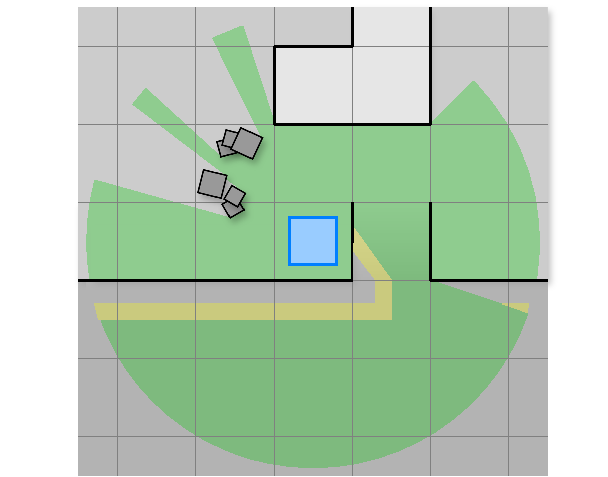
\includegraphics[width=\textwidth]{img/Range visualisation.pdf}
        Actual range.
    \end{minipage}%
    \begin{minipage}{.5\textwidth}
        \centering
        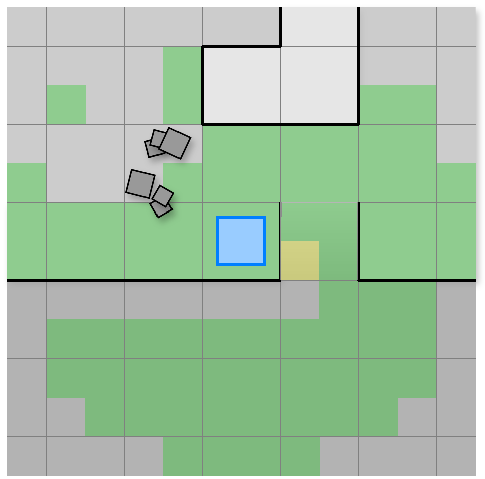
\includegraphics[width=0.8\textwidth]{img/range visualisation low res.pdf}\\
        Four samples per tile.
    \end{minipage}
    \caption{Range visualization approximation.}
    \label{fig:low-res-range}
\end{center}

So, for each special range type, we need an implementation of some sort of oracle that tells us for each point whether an attacker at that point would be visible or not.
For some towers, this oracle will perform a simple check whether the point lies within the range, but for others, more checks will be performed, notably the line of sight checks which are expensive.
Doing thousands of these point tests whenever the player selects a tower which performs line of sight checks would cause a noticeable stutter.
So, we will create a low-resolution visualization first, and slowly refine it by performing more tests over the next frames.

We will probably perform only few hundred line of sight checks per frame, and we don't want the visualization to keep changing for several seconds, so we will go with a rather small final resolution.
A grid of $256 \times 256$ squares, which is 65536 in total, should be enough, giving us $16 \times 16$ samples per tile.
The visualization will be obviously pixelated, but it should communicate the towers' range well.

We can build this visualization as a \emph{quadtree}~\cite{Quadtree}.
A quadtree is a data structure in the form of a rooted tree, where the root node represents the whole world as one large square, and each internal node has four children which split the parent node into four smaller squares.

We can start our visualization with the root node, and over time refine each leaf node by adding its four children.
For each child we perform a point test in its center and assign to it the obtained value.
This is repeated until all leaf nodes are of the required depth, which would be 8 for a $256 \times 256$ square grid.
Thus, we perform one third more point tests, but we can have a valid representation of the range after every frame that gets better over time.
This is illustrated in figures~\ref{fig:quadtree-1} and~\ref{fig:quadtree-11}.

\begin{center}
    \captionsetup{type=figure}
    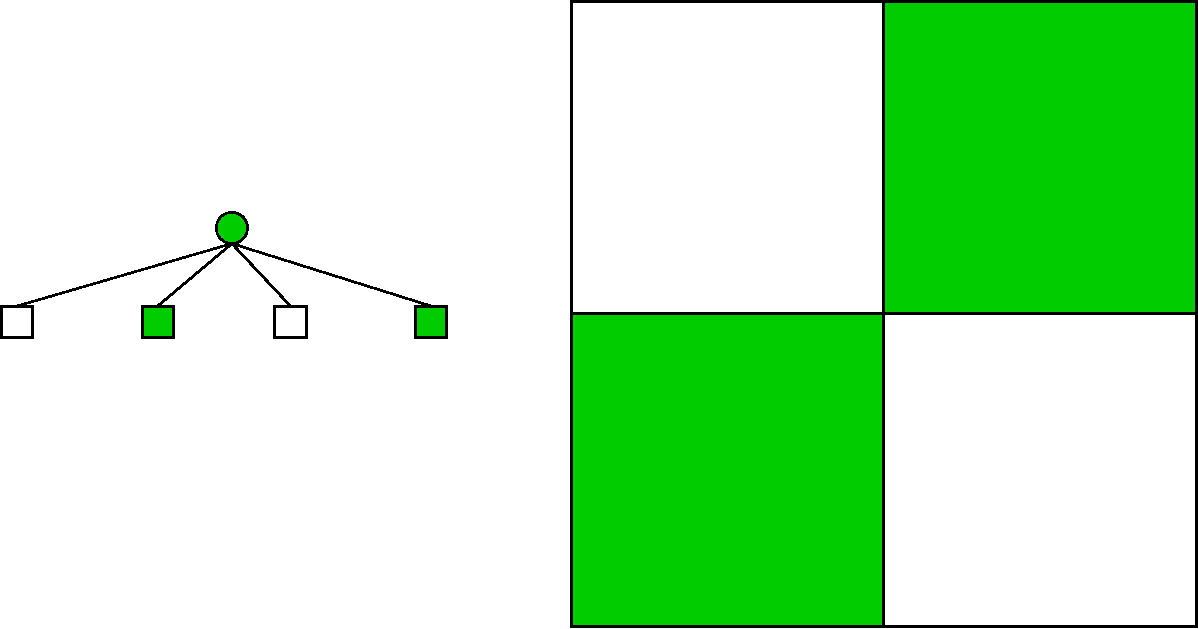
\includegraphics[width=0.8\textwidth]{img/quadtree 1.pdf}
    \caption{Quadtree range representation after expanding just the root node.}
    \label{fig:quadtree-1}
\end{center}

\begin{center}
    \captionsetup{type=figure}
    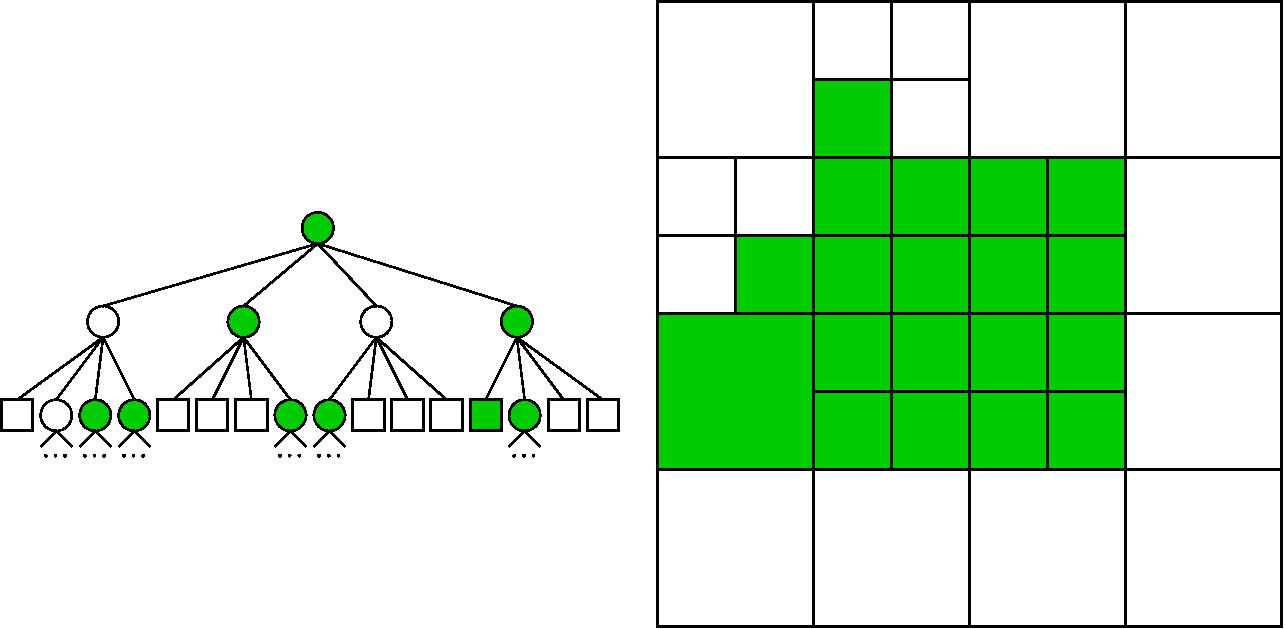
\includegraphics[width=0.8\textwidth]{img/quadtree 11.pdf}
    \caption{Quadtree range representation after expanding 11 nodes.}
    \label{fig:quadtree-11}
\end{center}

We can choose in which order to expand the leaf nodes by calculating a priority for each and storing unrefined nodes in a priority queue.
We should prioritize nodes which are larger, but also nodes whose siblings have different results than them, because this means they are near a boundary where the results change from one state to another.

This representation also lets us easily perform \emph{quadtree compression} to save memory:
Whenever all four children of an internal node match, and they are leaves that won't be refined further, we can delete them and mark their parent as also finished.
This can happen recursively, so that large squares with the same color can be represented by just one node.
This is illustrated in figures~\ref{fig:quadtree-full} and~\ref{fig:quadtree-compressed}.

\begin{center}
    \captionsetup{type=figure}
    \includegraphics[width=0.8\textwidth]{img/quadtree full.pdf}
    \caption{Quadtree range representation of a $16\times16$ grid of sample points.}
    \label{fig:quadtree-full}
\end{center}

\begin{center}
    \captionsetup{type=figure}
    \includegraphics[width=0.8\textwidth]{img/quadtree compressed.pdf}
    \caption{Compressed quadtree range representation.}
    \label{fig:quadtree-compressed}
\end{center}

Furthermore, we don't have to refine some nodes at all, when we know for sure that all points tests within their square will yield the same result.
To help with this, the point test oracles won't return only the result at that point, but also the guaranteed minimum distance to a point which gives a different result.
When the distance is greater than half of the current square's diagonal, we don't have to refine it further.
This distance is easy to determine for simple range shapes, but for towers with line of sight checks, it will always be reported as 0 for points inside the range.

\subsection{Representation for The GPU}

Now that we can compute the visualization, we also need to render it.
To do that, we need to send it to the GPU and display it using a shader.
But how do we represent it in the GPU?

The first option that comes to mind is to just take the quadtree we constructed and send it to the GPU.
Of course, we would have to put the data into some shader buffer, probably by creating an array of nodes.
We want to reduce the bandwidth as much as possible, so all children of a single node could be consecutive in the array, so each node would only need to store one index to the array to reference all its children.
Theoretically, we would need at most $4/3 \times 65535$ nodes in order to represent the $256 \times 256$ resolution we selected, but thanks to quadtree compression, we usually won't need as many.
So, each node could be represented by 2 bytes, since we only need to save one index to the children or the result of the point test for leaf nodes.

However, this approach is expensive on the CPU, because we need to prepare this data structure.
And on the GPU too, because it needs to traverse the tree to its leaf to determine the color for each pixel with the terrain, but that isn't as big of a problem, since overall, the GPU is much more powerful.

A better option might be to store the data directly in a texture.
In the GPU, we only have to access the texture once to determine the color of a given position on the terrain, making it much simpler.
On the CPU side, it will be simpler too.
For each node, we fill a square that is represented by it the texture with the value of the node, all the way to single pixels for the deepest nodes.

This is much better, but we can save some more CPU computation with a trick:
\emph{Mipmapping}, first described in the paper \citetitle{Mipmaps}~\cite{Mipmaps}, is a widely used technique where we generate several lower-resolution variants of a texture, which can then be used to reduce aliasing and performance cost when rendering surfaces from a great distance or when viewed at a shallow angle.
The width and height of each additional image is a half of the previous level.
These are usually automatically generated from the main texture, but we can make them look how we want, and we can use them how we want.

If we create a texture with mip levels all the way to a $1 \times 1$ image, and we imagine all the layers stacked on top of each other, stretched to be the same size as the terrain, we essentially get a quadtree.
The root node of our quadtree is the only pixel in the highest layer, and each other pixel represents another node, each in the layer corresponding to its depth, directly below its parent.
This is illustrated in figure~\ref{fig:quadtree-mipmap}.
Here we mark non-leaf nodes with red color and pixels with no corresponding nodes in blue.

Now, the CPU only has to change one pixel for each node.
However, the GPU has to access the texture multiple times per each pixel again, but that shouldn't be a problem.
Including the mipmaps also makes the texture one third larger than without them.
Whenever we change a part of a texture, it has to be copied to the GPU again.
Since we do this every frame, bandwidth will probably be the limiting factor, but for our small 87\,KiB texture this shouldn't be an issue.

\begin{center}
    \captionsetup{type=figure}
    \includegraphics[width=0.8\textwidth]{img/quadtree mipmaps.pdf}
    \caption{Quadtree stored in a mipmapped texture.}
    \label{fig:quadtree-mipmap}
\end{center}

\subsection{Computing Everything on the GPU}

We would like to mention that only after implementing the demo version of our game, we thought of a solution that can be used if higher resolution of the visualization is needed, or just to improve performance.
This is the exact kind of task that GPUs are great at: computing the same thing for many points at once.
So, it would be the best to only send the world geometry to the GPU, and compute these range visualizations there.
Testing which points are in the line of sight of some tower is the same, as if the tower was a point light, and we wanted to draw the shadows.
This is a problem that has been heavily studied and there are many techniques we could use for it.

\section{Blueprints and Info Panel Text}

In section~\ref{sec:design-blueprints} we described that in our game, the player will be able to build buildings or use abilities, only if they have their blueprint.
Each blueprint will include a description that explains its function, including the exact values of important statistics.

\subsection{Blueprint Representation}

We also mentioned that the blueprints will be modifiable, be it permanently or temporarily.
For example, we could have a building that increases the range of all buildings adjacent to it, or an augment that increases the damage of the blueprint it augments.
To do this, we would like to know from each blueprint whether it has a given statistic and its value.
It is also important to note that we want to access these statistics even without creating an instance of the thing the blueprint represents.
So, all the statistics we could ever want to know or modify will not be stored in the class that represents blueprints, separately from the implementation of their behavior.

In Unity, we will implement blueprints as \emph{scriptable objects}.
Unity allows us to edit the values of these in the editor, and to save them in the project as separate files.
We can also include references to other resources in our project, for example the \emph{prefab} of the object that get instantiated when the blueprint is used in a battle.
These prefabs are then where we put the scripts that implement the actual behavior of the building or ability.
The blueprint itself will only hold the stats and the description.
When the prefab is created, it will be assigned a copy of the blueprint, in order to have access to the blueprint statistics, which can be modified separately from the source blueprint.

Similarly, we will use scriptable objects to represent attacker types.
They will hold the stats and the description of the attacker type, and a reference to the prefab of the attacker itself.

\subsection{Info Panel Text}\label{sec:analysis-description-tags}
In section~\ref{sec:design-info-panel}, we describe that the information about anything the player has selected will be displayed on an info panel on the right side of the screen.
For blueprints, this will be mainly their statistics and the description.
For buildings, the info panel will display the up-to-date stats and description of their blueprint, but the buildings can also include some information of their own, for example, each tower will show the damage it has dealt throughout the battle.
We also specified that the statistics that have changed from the original blueprint will be highlighted using colors, indicating whether they changed for better or for the worse.
Additionally, any new or removed abilities will also be highlighted.

To dynamically update the statistics, we will use placeholder tags in the descriptions, and then a preprocessor, which will find these tags and replace them with the up-to-date values, including the correct formatting.
For example, the tag \mono{[DMG]} will be replaced by the damage statistic, correctly formatted, and prefixed with an icon that symbolizes the damage stat, to show that if something changes damage, this value will change.
Of course, to compare the new value, we will also need to store the original value.

To display this formatting and icons within text, we will use the features of the Unity package \emph{Text Mesh Pro}.
It lets us format the text with tags similar to HTML.
For the icons, we can create a \emph{Text Mesh Pro sprite asset}, and then insert the icons into the text using the tag \mono{<sprite=ID>}.

\section{Modifiable Commands and Queries}\label{sec:analysis-modifiable-commands}

In our game, we want various objects to modify how other objects function.
However, this can be very problematic if we don't select the right approach.

For example, we could have a building that slows down attackers in its range by 25\%, or an attacker that speeds up by 1 tile per second once its HP drops below half.
However, this can cause issues when implemented incorrectly:
Imagine the attacker that speeds up has a base speed of 1 tile per second.
Then, it enters the range of the building that slows it down to three quarters, dropping its speed to 0.75\,t/s.
Then its speed increases by 1\,t/s, because its HP drops, so the new speed is 1.75\,t/s, but we would expect it to be 1.5\,t/s.
Finally, when it leaves the range of the building, its speed increases by third of the current speed to revert the slowdown, ending up at 2.333 tiles per second.
This is obviously not equal to the expected speed of 2 tiles per second.
This situation is illustrated in figure~\ref{fig:speed-changes}.

\begin{center}
    \captionsetup{type=figure}
    \includegraphics[width=0.6\textwidth]{img/speed changes.pdf}
    \caption{Possible discrepancy when multiple effects change an attacker's speed.}
    \label{fig:speed-changes}
\end{center}

To illustrate another problem we might run into, we imagine a building that makes it so whenever the player would get energy, they get that many materials instead.
How would we implement it?
We obviously don't want to modify the blueprints of other buildings, and there might be other sources of energy too.
We could add a special case to the code that handles the player's current material and energy balance to check specifically for this building, and handle the conversion if needed.
That cannot be a good solution.
Furthermore, the sources of the energy would still show pop-ups that they produced some energy, even though they produced materials instead.

\subsection{Modifiable Commands}

Our solution for these issues is what we call \emph{modifiable commands and queries}.
This system is an extension of the \emph{observer pattern}~\cite{Observer}.
In this pattern, many \emph{subscribers} can subscribe to an \emph{event}, to be notified when the event occurs.
This event can be triggered by any other object that has a reference to it, also known as \emph{publisher}.
The advantage of this pattern is its weak coupling.
The subscribers don't have to know anything about other subscribers or about the publishers and vice versa.

To create modifiable commands, we add the option for subscribers to modify the data of the event, and we invoke the subscribers' callbacks in an order based on the priority that was specified when they subscribed to the command.
For example, when a building wants to produce energy, it invokes the modifiable command to add the given amount of energy.
The command then notifies all the registered modifiers' callbacks, one by one.
Each subscriber alters the amount of energy how it wants, and finally, the last subscriber, which we'll call the \emph{handler}, reads the energy amount and adds it to the total.
The handler also doesn't have to be the last subscriber, there can be more subscribers after it which react to the event, for example by displaying the amount produced.
We will call these \emph{reactions}, and we will refer to the subscribers that get notified before the handler as \emph{modifiers}.
We will also let modifiers cancel the command completely.

This is illustrated in figure~\ref{fig:modifiable-command}.
It shows an example of a command to add energy.
A solar panel produces tries to produce 10 energy, but the energy amplifier has registered a modifier which increases it to 15.
The player state handles this command by adding the energy to the player's energy amount.
Finally, reactions are notified, in this case a reaction to show the number and one to play the sound.

\begin{center}
    \captionsetup{type=figure}
    \includegraphics[width=\textwidth]{img/modifiable command.pdf}
    \caption{Modifiable command to add energy.}
    \label{fig:modifiable-command}
\end{center}

It doesn't make sense to have more than one handler for the command, so we will say that the handles always has priority 0, and there can only ever be one.
The reactions shouldn't need to modify the command anymore, since it has already been handled by the handler, so we don't let them modify the command, only react to it.
This means the signature of their callback will be different, and they will be registered separately from the modifiers.
We will also force callbacks registered as a reaction to have a positive priority, so they happen after the handler.
And that leaves negative priority values for modifiers.

It is now easy to see how we would implement the example building that turns energy into materials.
It would simply register a modifier to the command for producing energy, which would cancel the command and invoke a command to produce materials instead.

\subsection{Modifiable Queries}

We could solve the first example with the attacker speed similarly.
Instead of just reading the speed value from the attacker stats, we will have a modifiable command for reading it.
So, when anyone wants to know the attacker's speed, they invoke the command with the base speed 1 as the initial data, and after series of modifications, they handle the updated value.
This ensures that multiple simultaneous modifiers don't produce an invalid value, and the order of application no longer matters, because they are ordered by their priority.

However, we don't ever need to react to a query, furthermore it would make no sense for a modifier to cancel a query.
Also, it makes no sense to handle the result using a callback that is then immediately unsubscribed.
So, we remove these features and streamline the interface to get \emph{modifiable queries}.

A modifiable command is invoked with some initial parameter that can be modified.
This doesn't make sense for a query.
If we query the speed of an attacker, we call the query with the attacker as an input, and the result is the attacker's speed.
To achieve this, we register a \emph{provider} which acquires the base value from the input, before both the input and the value are sent through the modifiers.

In figure~\ref{fig:modifiable-query}, we show a query that determines the speed of the attacker in the example at the beginning of section~\ref{sec:analysis-modifiable-commands}.
In the depicted situation, the attacker is in range of the slowing building, and also below half HP.
To determine the speed, first, this query's provider determines the base speed.
It is then modified by the attacker's ability, and by the slowing building.
Both of these modifiers use the attacker reference to determine whether they should apply or not, since the slowing building only slows down attackers in range, and the attacker's ability only applies to attackers below half HP.

\begin{center}
    \captionsetup{type=figure}
    \includegraphics[width=\textwidth]{img/modifiable query.pdf}
    \caption{Modifiable query for determining attacker speed.}
    \label{fig:modifiable-query}
\end{center}

\subsection{Event Reaction Chain}

For modifiable queries, we used only the first half of the modifiable command pipeline.
If we take just the second half, we get an event system, but with reactions ordered by priority.
This is also useful for us, because the reactions could create race conditions if their order wasn't fixed.
We call this the \emph{event reaction chain} just to differentiate it from Unity events, Unity event system and .NET events.